\documentclass{whiteboard}
\begin{document}
\begin{frame}[plain,t]
\bbcover{Grafos}{Algoritmo de Kosaraju}{Prof. Edson Alves}{Faculdade UnB Gama}

\end{frame}
\begin{frame}[plain,t]
\begin{tikzpicture}
\node[draw,opacity=0] at (0, 0) {x};
\node[draw,opacity=0] at (14, 8) {x};

	\node[anchor=west] (title) at (0.0, 7.0) { \Large \bbbold{Proponente} };

	\node[] (kosaraju) at (7.0, 4.0) { \includegraphics[scale=0.6]{figs/kosaraju.jpeg} };

	\node[] (kname) at (7.0, 1.0) { \bbbold{S. Rao Kosaraju} };

	\node[] (kdate) at (7.0, 0.5) { \bbtext{(1978)} };

\end{tikzpicture}
\end{frame}
\begin{frame}[plain,t]
\begin{tikzpicture}
\node[draw,opacity=0] at (0, 0) {x};
\node[draw,opacity=0] at (14, 8) {x};

	\node[anchor=west] (title) at (0.0, 6.5) { \Large \bbbold{Características do algoritmo de Kosaraju} };
\end{tikzpicture}
\end{frame}
\begin{frame}[plain,t]
\begin{tikzpicture}
\node[draw,opacity=0] at (0, 0) {x};
\node[draw,opacity=0] at (14, 8) {x};

	\node[anchor=west] (title) at (0.0, 6.5) { \Large \bbbold{Características do algoritmo de Kosaraju} };

	\node[anchor=west] (a) at (1.0, 5.5) { $\star$ \bbtext{O algoritmo de Kosaraju encontra os componentes fortemente conectados} };

	\node[anchor=west] (a1) at (0.5, 4.75) { \bbtext{de um grafo direcionado} };

\end{tikzpicture}
\end{frame}
\begin{frame}[plain,t]
\begin{tikzpicture}
\node[draw,opacity=0] at (0, 0) {x};
\node[draw,opacity=0] at (14, 8) {x};

	\node[anchor=west] (title) at (0.0, 6.5) { \Large \bbbold{Características do algoritmo de Kosaraju} };

	\node[anchor=west] (a) at (1.0, 5.5) { $\star$ \bbtext{O algoritmo de Kosaraju encontra os componentes fortemente conectados} };

	\node[anchor=west] (a1) at (0.5, 4.75) { \bbtext{de um grafo direcionado} };


	\node[anchor=west] (b) at (1.0, 3.75) { $\star$ \bbtext{O algoritmo realiza duas buscas em profundidade} };

\end{tikzpicture}
\end{frame}
\begin{frame}[plain,t]
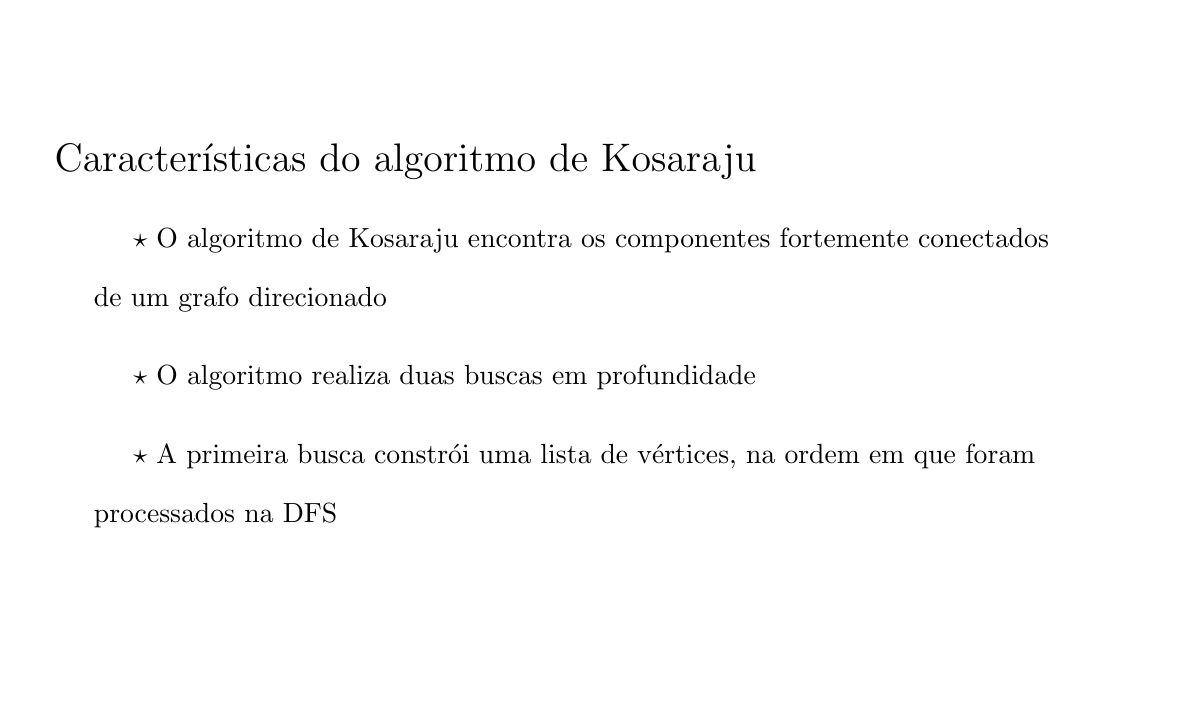
\begin{tikzpicture}
\node[draw,opacity=0] at (0, 0) {x};
\node[draw,opacity=0] at (14, 8) {x};

	\node[anchor=west] (title) at (0.0, 6.5) { \Large \bbbold{Características do algoritmo de Kosaraju} };

	\node[anchor=west] (a) at (1.0, 5.5) { $\star$ \bbtext{O algoritmo de Kosaraju encontra os componentes fortemente conectados} };

	\node[anchor=west] (a1) at (0.5, 4.75) { \bbtext{de um grafo direcionado} };


	\node[anchor=west] (b) at (1.0, 3.75) { $\star$ \bbtext{O algoritmo realiza duas buscas em profundidade} };


	\node[anchor=west] (c) at (1.0, 2.75) { $\star$ \bbtext{A primeira busca constrói uma lista de vértices, na ordem em que foram} };

	\node[anchor=west] (c1) at (0.5, 2.0) { \bbtext{processados na DFS} };


\end{tikzpicture}
\end{frame}
\begin{frame}[plain,t]
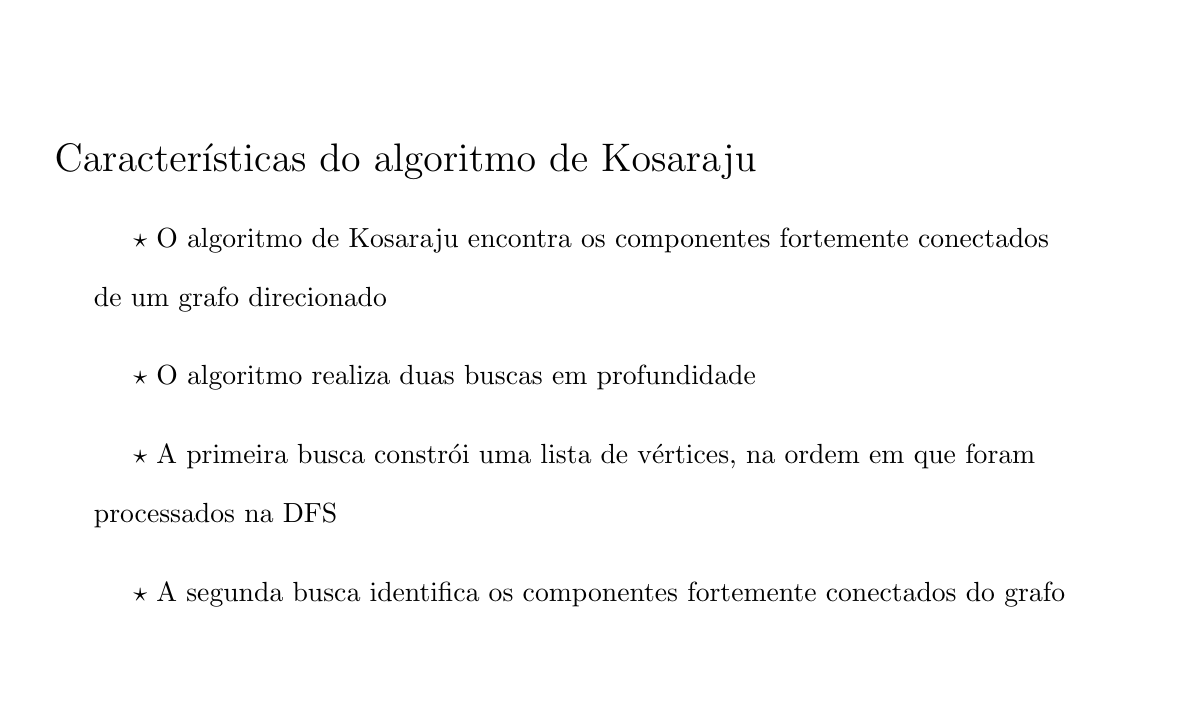
\begin{tikzpicture}
\node[draw,opacity=0] at (0, 0) {x};
\node[draw,opacity=0] at (14, 8) {x};

	\node[anchor=west] (title) at (0.0, 6.5) { \Large \bbbold{Características do algoritmo de Kosaraju} };

	\node[anchor=west] (a) at (1.0, 5.5) { $\star$ \bbtext{O algoritmo de Kosaraju encontra os componentes fortemente conectados} };

	\node[anchor=west] (a1) at (0.5, 4.75) { \bbtext{de um grafo direcionado} };


	\node[anchor=west] (b) at (1.0, 3.75) { $\star$ \bbtext{O algoritmo realiza duas buscas em profundidade} };


	\node[anchor=west] (c) at (1.0, 2.75) { $\star$ \bbtext{A primeira busca constrói uma lista de vértices, na ordem em que foram} };

	\node[anchor=west] (c1) at (0.5, 2.0) { \bbtext{processados na DFS} };



	\node[anchor=west] (d) at (1.0, 1.0) { $\star$ \bbtext{A segunda busca identifica os componentes fortemente conectados do grafo} };


\end{tikzpicture}
\end{frame}
\begin{frame}[plain,t]
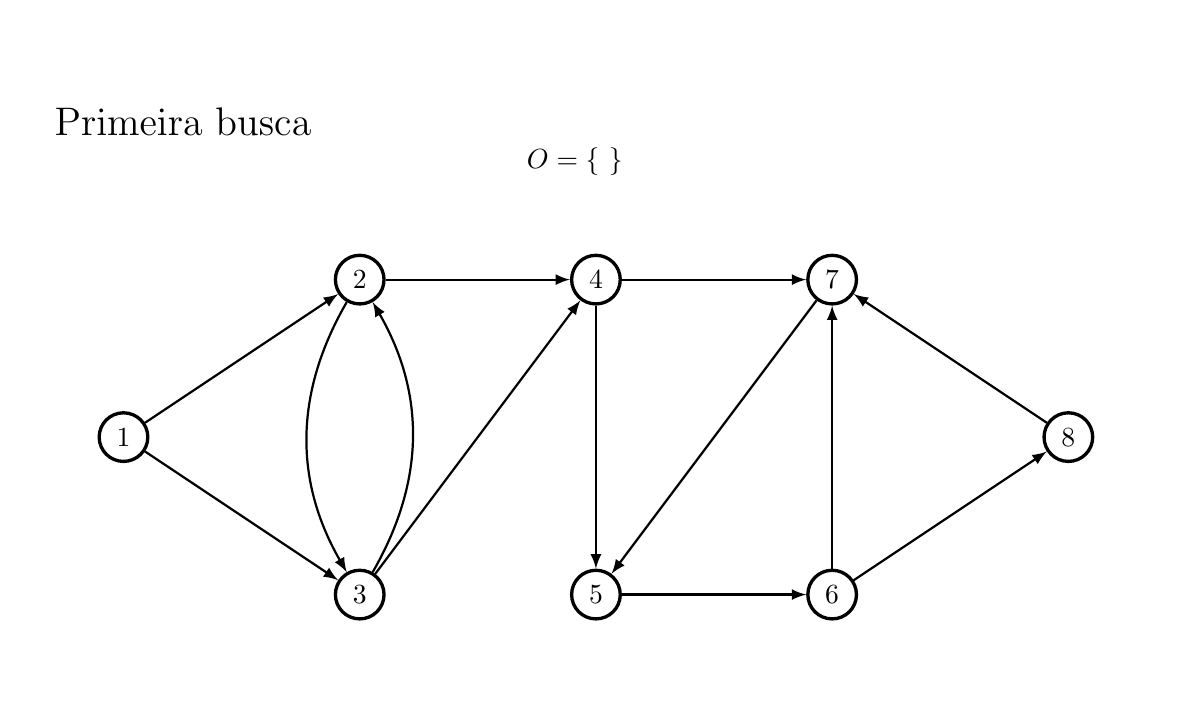
\begin{tikzpicture}
\node[draw,opacity=0] at (0, 0) {x};
\node[draw,opacity=0] at (14, 8) {x};

	\node[anchor=west] (title) at (0.0, 7.0) { \Large \bbbold{Primeira busca} };

	\node[anchor=west] (order) at (6.0, 6.5) { $O = \{\ \}$ };


	\node[very thick,draw,circle] (node1) at (1.0, 3.0) { \bbtext{1} };

	\node[very thick,draw,circle] (node2) at (4.0, 5.0) { \bbtext{2} };

	\node[very thick,draw,circle] (node3) at (4.0, 1.0) { \bbtext{3} };

	\node[very thick,draw,circle] (node4) at (7.0, 5.0) { \bbtext{4} };

	\node[very thick,draw,circle] (node5) at (7.0, 1.0) { \bbtext{5} };

	\node[very thick,draw,circle] (node7) at (10.0, 5.0) { \bbtext{7} };

	\node[very thick,draw,circle] (node6) at (10.0, 1.0) { \bbtext{6} };

	\node[very thick,draw,circle] (node8) at (13.0, 3.0) { \bbtext{8} };

	\draw[thick,-latex](node1) to (node2);

	\draw[thick,-latex](node1) to (node3);

	\draw[thick,-latex](node3) to [bend right] (node2);

	\draw[thick,-latex](node2) to [bend right] (node3);

	\draw[thick,-latex](node2) to (node4);

	\draw[thick,-latex](node3) to (node4);

	\draw[thick,-latex](node4) to (node5);

	\draw[thick,-latex](node4) to (node7);

	\draw[thick,-latex](node5) to (node6);

	\draw[thick,-latex](node6) to (node7);

	\draw[thick,-latex](node6) to (node8);

	\draw[thick,-latex](node7) to (node5);

	\draw[thick,-latex](node8) to (node7);

\end{tikzpicture}
\end{frame}
\begin{frame}[plain,t]
\begin{tikzpicture}
\node[draw,opacity=0] at (0, 0) {x};
\node[draw,opacity=0] at (14, 8) {x};

	\node[anchor=west] (title) at (0.0, 7.0) { \Large \bbbold{Primeira busca} };

	\node[anchor=west] (order) at (6.0, 6.5) { $O = \{\ \}$ };


	\node[very thick,draw,circle,fill=BBGreen] (node1) at (1.0, 3.0) { \bbtext{1} };

	\node[very thick,draw,circle] (node2) at (4.0, 5.0) { \bbtext{2} };

	\node[very thick,draw,circle] (node3) at (4.0, 1.0) { \bbtext{3} };

	\node[very thick,draw,circle] (node4) at (7.0, 5.0) { \bbtext{4} };

	\node[very thick,draw,circle] (node5) at (7.0, 1.0) { \bbtext{5} };

	\node[very thick,draw,circle] (node7) at (10.0, 5.0) { \bbtext{7} };

	\node[very thick,draw,circle] (node6) at (10.0, 1.0) { \bbtext{6} };

	\node[very thick,draw,circle] (node8) at (13.0, 3.0) { \bbtext{8} };

	\draw[thick,-latex](node1) to (node2);

	\draw[thick,-latex](node1) to (node3);

	\draw[thick,-latex](node3) to [bend right] (node2);

	\draw[thick,-latex](node2) to [bend right] (node3);

	\draw[thick,-latex](node2) to (node4);

	\draw[thick,-latex](node3) to (node4);

	\draw[thick,-latex](node4) to (node5);

	\draw[thick,-latex](node4) to (node7);

	\draw[thick,-latex](node5) to (node6);

	\draw[thick,-latex](node6) to (node7);

	\draw[thick,-latex](node6) to (node8);

	\draw[thick,-latex](node7) to (node5);

	\draw[thick,-latex](node8) to (node7);


\end{tikzpicture}
\end{frame}
\begin{frame}[plain,t]
\begin{tikzpicture}
\node[draw,opacity=0] at (0, 0) {x};
\node[draw,opacity=0] at (14, 8) {x};

	\node[anchor=west] (title) at (0.0, 7.0) { \Large \bbbold{Primeira busca} };

	\node[anchor=west] (order) at (6.0, 6.5) { $O = \{\ \}$ };


	\node[very thick,draw,circle,fill=BBGreen] (node1) at (1.0, 3.0) { \bbtext{1} };

	\node[very thick,draw,circle,fill=BBGreen] (node2) at (4.0, 5.0) { \bbtext{2} };

	\node[very thick,draw,circle] (node3) at (4.0, 1.0) { \bbtext{3} };

	\node[very thick,draw,circle] (node4) at (7.0, 5.0) { \bbtext{4} };

	\node[very thick,draw,circle] (node5) at (7.0, 1.0) { \bbtext{5} };

	\node[very thick,draw,circle] (node7) at (10.0, 5.0) { \bbtext{7} };

	\node[very thick,draw,circle] (node6) at (10.0, 1.0) { \bbtext{6} };

	\node[very thick,draw,circle] (node8) at (13.0, 3.0) { \bbtext{8} };

	\draw[thick,-latex](node1) to (node2);

	\draw[thick,-latex](node1) to (node3);

	\draw[thick,-latex](node3) to [bend right] (node2);

	\draw[thick,-latex](node2) to [bend right] (node3);

	\draw[thick,-latex](node2) to (node4);

	\draw[thick,-latex](node3) to (node4);

	\draw[thick,-latex](node4) to (node5);

	\draw[thick,-latex](node4) to (node7);

	\draw[thick,-latex](node5) to (node6);

	\draw[thick,-latex](node6) to (node7);

	\draw[thick,-latex](node6) to (node8);

	\draw[thick,-latex](node7) to (node5);

	\draw[thick,-latex](node8) to (node7);



\end{tikzpicture}
\end{frame}
\begin{frame}[plain,t]
\begin{tikzpicture}
\node[draw,opacity=0] at (0, 0) {x};
\node[draw,opacity=0] at (14, 8) {x};

	\node[anchor=west] (title) at (0.0, 7.0) { \Large \bbbold{Primeira busca} };

	\node[anchor=west] (order) at (6.0, 6.5) { $O = \{\ \}$ };


	\node[very thick,draw,circle,fill=BBGreen] (node1) at (1.0, 3.0) { \bbtext{1} };

	\node[very thick,draw,circle,fill=BBGreen] (node2) at (4.0, 5.0) { \bbtext{2} };

	\node[very thick,draw,circle,fill=BBGreen] (node3) at (4.0, 1.0) { \bbtext{3} };

	\node[very thick,draw,circle] (node4) at (7.0, 5.0) { \bbtext{4} };

	\node[very thick,draw,circle] (node5) at (7.0, 1.0) { \bbtext{5} };

	\node[very thick,draw,circle] (node7) at (10.0, 5.0) { \bbtext{7} };

	\node[very thick,draw,circle] (node6) at (10.0, 1.0) { \bbtext{6} };

	\node[very thick,draw,circle] (node8) at (13.0, 3.0) { \bbtext{8} };

	\draw[thick,-latex](node1) to (node2);

	\draw[thick,-latex](node1) to (node3);

	\draw[thick,-latex](node3) to [bend right] (node2);

	\draw[thick,-latex](node2) to [bend right] (node3);

	\draw[thick,-latex](node2) to (node4);

	\draw[thick,-latex](node3) to (node4);

	\draw[thick,-latex](node4) to (node5);

	\draw[thick,-latex](node4) to (node7);

	\draw[thick,-latex](node5) to (node6);

	\draw[thick,-latex](node6) to (node7);

	\draw[thick,-latex](node6) to (node8);

	\draw[thick,-latex](node7) to (node5);

	\draw[thick,-latex](node8) to (node7);




\end{tikzpicture}
\end{frame}
\begin{frame}[plain,t]
\begin{tikzpicture}
\node[draw,opacity=0] at (0, 0) {x};
\node[draw,opacity=0] at (14, 8) {x};

	\node[anchor=west] (title) at (0.0, 7.0) { \Large \bbbold{Primeira busca} };

	\node[anchor=west] (order) at (6.0, 6.5) { $O = \{\ \}$ };


	\node[very thick,draw,circle,fill=BBGreen] (node1) at (1.0, 3.0) { \bbtext{1} };

	\node[very thick,draw,circle,fill=BBGreen] (node2) at (4.0, 5.0) { \bbtext{2} };

	\node[very thick,draw,circle,fill=BBGreen] (node3) at (4.0, 1.0) { \bbtext{3} };

	\node[very thick,draw,circle,fill=BBGreen] (node4) at (7.0, 5.0) { \bbtext{4} };

	\node[very thick,draw,circle] (node5) at (7.0, 1.0) { \bbtext{5} };

	\node[very thick,draw,circle] (node7) at (10.0, 5.0) { \bbtext{7} };

	\node[very thick,draw,circle] (node6) at (10.0, 1.0) { \bbtext{6} };

	\node[very thick,draw,circle] (node8) at (13.0, 3.0) { \bbtext{8} };

	\draw[thick,-latex](node1) to (node2);

	\draw[thick,-latex](node1) to (node3);

	\draw[thick,-latex](node3) to [bend right] (node2);

	\draw[thick,-latex](node2) to [bend right] (node3);

	\draw[thick,-latex](node2) to (node4);

	\draw[thick,-latex](node3) to (node4);

	\draw[thick,-latex](node4) to (node5);

	\draw[thick,-latex](node4) to (node7);

	\draw[thick,-latex](node5) to (node6);

	\draw[thick,-latex](node6) to (node7);

	\draw[thick,-latex](node6) to (node8);

	\draw[thick,-latex](node7) to (node5);

	\draw[thick,-latex](node8) to (node7);





\end{tikzpicture}
\end{frame}
\begin{frame}[plain,t]
\begin{tikzpicture}
\node[draw,opacity=0] at (0, 0) {x};
\node[draw,opacity=0] at (14, 8) {x};

	\node[anchor=west] (title) at (0.0, 7.0) { \Large \bbbold{Primeira busca} };

	\node[anchor=west] (order) at (6.0, 6.5) { $O = \{\ \}$ };


	\node[very thick,draw,circle,fill=BBGreen] (node1) at (1.0, 3.0) { \bbtext{1} };

	\node[very thick,draw,circle,fill=BBGreen] (node2) at (4.0, 5.0) { \bbtext{2} };

	\node[very thick,draw,circle,fill=BBGreen] (node3) at (4.0, 1.0) { \bbtext{3} };

	\node[very thick,draw,circle,fill=BBGreen] (node4) at (7.0, 5.0) { \bbtext{4} };

	\node[very thick,draw,circle,fill=BBGreen] (node5) at (7.0, 1.0) { \bbtext{5} };

	\node[very thick,draw,circle] (node7) at (10.0, 5.0) { \bbtext{7} };

	\node[very thick,draw,circle] (node6) at (10.0, 1.0) { \bbtext{6} };

	\node[very thick,draw,circle] (node8) at (13.0, 3.0) { \bbtext{8} };

	\draw[thick,-latex](node1) to (node2);

	\draw[thick,-latex](node1) to (node3);

	\draw[thick,-latex](node3) to [bend right] (node2);

	\draw[thick,-latex](node2) to [bend right] (node3);

	\draw[thick,-latex](node2) to (node4);

	\draw[thick,-latex](node3) to (node4);

	\draw[thick,-latex](node4) to (node5);

	\draw[thick,-latex](node4) to (node7);

	\draw[thick,-latex](node5) to (node6);

	\draw[thick,-latex](node6) to (node7);

	\draw[thick,-latex](node6) to (node8);

	\draw[thick,-latex](node7) to (node5);

	\draw[thick,-latex](node8) to (node7);






\end{tikzpicture}
\end{frame}
\begin{frame}[plain,t]
\begin{tikzpicture}
\node[draw,opacity=0] at (0, 0) {x};
\node[draw,opacity=0] at (14, 8) {x};

	\node[anchor=west] (title) at (0.0, 7.0) { \Large \bbbold{Primeira busca} };

	\node[anchor=west] (order) at (6.0, 6.5) { $O = \{\ \}$ };


	\node[very thick,draw,circle,fill=BBGreen] (node1) at (1.0, 3.0) { \bbtext{1} };

	\node[very thick,draw,circle,fill=BBGreen] (node2) at (4.0, 5.0) { \bbtext{2} };

	\node[very thick,draw,circle,fill=BBGreen] (node3) at (4.0, 1.0) { \bbtext{3} };

	\node[very thick,draw,circle,fill=BBGreen] (node4) at (7.0, 5.0) { \bbtext{4} };

	\node[very thick,draw,circle,fill=BBGreen] (node5) at (7.0, 1.0) { \bbtext{5} };

	\node[very thick,draw,circle] (node7) at (10.0, 5.0) { \bbtext{7} };

	\node[very thick,draw,circle,fill=BBGreen] (node6) at (10.0, 1.0) { \bbtext{6} };

	\node[very thick,draw,circle] (node8) at (13.0, 3.0) { \bbtext{8} };

	\draw[thick,-latex](node1) to (node2);

	\draw[thick,-latex](node1) to (node3);

	\draw[thick,-latex](node3) to [bend right] (node2);

	\draw[thick,-latex](node2) to [bend right] (node3);

	\draw[thick,-latex](node2) to (node4);

	\draw[thick,-latex](node3) to (node4);

	\draw[thick,-latex](node4) to (node5);

	\draw[thick,-latex](node4) to (node7);

	\draw[thick,-latex](node5) to (node6);

	\draw[thick,-latex](node6) to (node7);

	\draw[thick,-latex](node6) to (node8);

	\draw[thick,-latex](node7) to (node5);

	\draw[thick,-latex](node8) to (node7);







\end{tikzpicture}
\end{frame}
\begin{frame}[plain,t]
\begin{tikzpicture}
\node[draw,opacity=0] at (0, 0) {x};
\node[draw,opacity=0] at (14, 8) {x};

	\node[anchor=west] (title) at (0.0, 7.0) { \Large \bbbold{Primeira busca} };

	\node[anchor=west] (order) at (6.0, 6.5) { $O = \{\ \}$ };


	\node[very thick,draw,circle,fill=BBGreen] (node1) at (1.0, 3.0) { \bbtext{1} };

	\node[very thick,draw,circle,fill=BBGreen] (node2) at (4.0, 5.0) { \bbtext{2} };

	\node[very thick,draw,circle,fill=BBGreen] (node3) at (4.0, 1.0) { \bbtext{3} };

	\node[very thick,draw,circle,fill=BBGreen] (node4) at (7.0, 5.0) { \bbtext{4} };

	\node[very thick,draw,circle,fill=BBGreen] (node5) at (7.0, 1.0) { \bbtext{5} };

	\node[very thick,draw,circle] (node7) at (10.0, 5.0) { \bbtext{7} };

	\node[very thick,draw,circle,fill=BBGreen] (node6) at (10.0, 1.0) { \bbtext{6} };

	\node[very thick,draw,circle,fill=BBGreen] (node8) at (13.0, 3.0) { \bbtext{8} };

	\draw[thick,-latex](node1) to (node2);

	\draw[thick,-latex](node1) to (node3);

	\draw[thick,-latex](node3) to [bend right] (node2);

	\draw[thick,-latex](node2) to [bend right] (node3);

	\draw[thick,-latex](node2) to (node4);

	\draw[thick,-latex](node3) to (node4);

	\draw[thick,-latex](node4) to (node5);

	\draw[thick,-latex](node4) to (node7);

	\draw[thick,-latex](node5) to (node6);

	\draw[thick,-latex](node6) to (node7);

	\draw[thick,-latex](node6) to (node8);

	\draw[thick,-latex](node7) to (node5);

	\draw[thick,-latex](node8) to (node7);








\end{tikzpicture}
\end{frame}
\begin{frame}[plain,t]
\begin{tikzpicture}
\node[draw,opacity=0] at (0, 0) {x};
\node[draw,opacity=0] at (14, 8) {x};

	\node[anchor=west] (title) at (0.0, 7.0) { \Large \bbbold{Primeira busca} };

	\node[anchor=west] (order) at (6.0, 6.5) { $O = \{\ \}$ };


	\node[very thick,draw,circle,fill=BBGreen] (node1) at (1.0, 3.0) { \bbtext{1} };

	\node[very thick,draw,circle,fill=BBGreen] (node2) at (4.0, 5.0) { \bbtext{2} };

	\node[very thick,draw,circle,fill=BBGreen] (node3) at (4.0, 1.0) { \bbtext{3} };

	\node[very thick,draw,circle,fill=BBGreen] (node4) at (7.0, 5.0) { \bbtext{4} };

	\node[very thick,draw,circle,fill=BBGreen] (node5) at (7.0, 1.0) { \bbtext{5} };

	\node[very thick,draw,circle,fill=BBGreen] (node7) at (10.0, 5.0) { \bbtext{7} };

	\node[very thick,draw,circle,fill=BBGreen] (node6) at (10.0, 1.0) { \bbtext{6} };

	\node[very thick,draw,circle,fill=BBGreen] (node8) at (13.0, 3.0) { \bbtext{8} };

	\draw[thick,-latex](node1) to (node2);

	\draw[thick,-latex](node1) to (node3);

	\draw[thick,-latex](node3) to [bend right] (node2);

	\draw[thick,-latex](node2) to [bend right] (node3);

	\draw[thick,-latex](node2) to (node4);

	\draw[thick,-latex](node3) to (node4);

	\draw[thick,-latex](node4) to (node5);

	\draw[thick,-latex](node4) to (node7);

	\draw[thick,-latex](node5) to (node6);

	\draw[thick,-latex](node6) to (node7);

	\draw[thick,-latex](node6) to (node8);

	\draw[thick,-latex](node7) to (node5);

	\draw[thick,-latex](node8) to (node7);









\end{tikzpicture}
\end{frame}
\begin{frame}[plain,t]
\begin{tikzpicture}
\node[draw,opacity=0] at (0, 0) {x};
\node[draw,opacity=0] at (14, 8) {x};

	\node[anchor=west] (title) at (0.0, 7.0) { \Large \bbbold{Primeira busca} };

	\node[anchor=west] (order) at (6.0, 6.5) { $O = \{\ 7\ \}$ };


	\node[very thick,draw,circle,fill=BBGreen] (node1) at (1.0, 3.0) { \bbtext{1} };

	\node[very thick,draw,circle,fill=BBGreen] (node2) at (4.0, 5.0) { \bbtext{2} };

	\node[very thick,draw,circle,fill=BBGreen] (node3) at (4.0, 1.0) { \bbtext{3} };

	\node[very thick,draw,circle,fill=BBGreen] (node4) at (7.0, 5.0) { \bbtext{4} };

	\node[very thick,draw,circle,fill=BBGreen] (node5) at (7.0, 1.0) { \bbtext{5} };

	\node[very thick,draw,circle,fill=BBCyan] (node7) at (10.0, 5.0) { \bbtext{7} };

	\node[very thick,draw,circle,fill=BBGreen] (node6) at (10.0, 1.0) { \bbtext{6} };

	\node[very thick,draw,circle,fill=BBGreen] (node8) at (13.0, 3.0) { \bbtext{8} };

	\draw[thick,-latex](node1) to (node2);

	\draw[thick,-latex](node1) to (node3);

	\draw[thick,-latex](node3) to [bend right] (node2);

	\draw[thick,-latex](node2) to [bend right] (node3);

	\draw[thick,-latex](node2) to (node4);

	\draw[thick,-latex](node3) to (node4);

	\draw[thick,-latex](node4) to (node5);

	\draw[thick,-latex](node4) to (node7);

	\draw[thick,-latex](node5) to (node6);

	\draw[thick,-latex](node6) to (node7);

	\draw[thick,-latex](node6) to (node8);

	\draw[thick,-latex](node7) to (node5);

	\draw[thick,-latex](node8) to (node7);










\end{tikzpicture}
\end{frame}
\begin{frame}[plain,t]
\begin{tikzpicture}
\node[draw,opacity=0] at (0, 0) {x};
\node[draw,opacity=0] at (14, 8) {x};

	\node[anchor=west] (title) at (0.0, 7.0) { \Large \bbbold{Primeira busca} };

	\node[anchor=west] (order) at (6.0, 6.5) { $O = \{\ 7, 8\ \}$ };


	\node[very thick,draw,circle,fill=BBGreen] (node1) at (1.0, 3.0) { \bbtext{1} };

	\node[very thick,draw,circle,fill=BBGreen] (node2) at (4.0, 5.0) { \bbtext{2} };

	\node[very thick,draw,circle,fill=BBGreen] (node3) at (4.0, 1.0) { \bbtext{3} };

	\node[very thick,draw,circle,fill=BBGreen] (node4) at (7.0, 5.0) { \bbtext{4} };

	\node[very thick,draw,circle,fill=BBGreen] (node5) at (7.0, 1.0) { \bbtext{5} };

	\node[very thick,draw,circle,fill=BBCyan] (node7) at (10.0, 5.0) { \bbtext{7} };

	\node[very thick,draw,circle,fill=BBGreen] (node6) at (10.0, 1.0) { \bbtext{6} };

	\node[very thick,draw,circle,fill=BBCyan] (node8) at (13.0, 3.0) { \bbtext{8} };

	\draw[thick,-latex](node1) to (node2);

	\draw[thick,-latex](node1) to (node3);

	\draw[thick,-latex](node3) to [bend right] (node2);

	\draw[thick,-latex](node2) to [bend right] (node3);

	\draw[thick,-latex](node2) to (node4);

	\draw[thick,-latex](node3) to (node4);

	\draw[thick,-latex](node4) to (node5);

	\draw[thick,-latex](node4) to (node7);

	\draw[thick,-latex](node5) to (node6);

	\draw[thick,-latex](node6) to (node7);

	\draw[thick,-latex](node6) to (node8);

	\draw[thick,-latex](node7) to (node5);

	\draw[thick,-latex](node8) to (node7);











\end{tikzpicture}
\end{frame}
\begin{frame}[plain,t]
\begin{tikzpicture}
\node[draw,opacity=0] at (0, 0) {x};
\node[draw,opacity=0] at (14, 8) {x};

	\node[anchor=west] (title) at (0.0, 7.0) { \Large \bbbold{Primeira busca} };

	\node[anchor=west] (order) at (6.0, 6.5) { $O = \{\ 7, 8, 6\ \}$ };


	\node[very thick,draw,circle,fill=BBGreen] (node1) at (1.0, 3.0) { \bbtext{1} };

	\node[very thick,draw,circle,fill=BBGreen] (node2) at (4.0, 5.0) { \bbtext{2} };

	\node[very thick,draw,circle,fill=BBGreen] (node3) at (4.0, 1.0) { \bbtext{3} };

	\node[very thick,draw,circle,fill=BBGreen] (node4) at (7.0, 5.0) { \bbtext{4} };

	\node[very thick,draw,circle,fill=BBGreen] (node5) at (7.0, 1.0) { \bbtext{5} };

	\node[very thick,draw,circle,fill=BBCyan] (node7) at (10.0, 5.0) { \bbtext{7} };

	\node[very thick,draw,circle,fill=BBCyan] (node6) at (10.0, 1.0) { \bbtext{6} };

	\node[very thick,draw,circle,fill=BBCyan] (node8) at (13.0, 3.0) { \bbtext{8} };

	\draw[thick,-latex](node1) to (node2);

	\draw[thick,-latex](node1) to (node3);

	\draw[thick,-latex](node3) to [bend right] (node2);

	\draw[thick,-latex](node2) to [bend right] (node3);

	\draw[thick,-latex](node2) to (node4);

	\draw[thick,-latex](node3) to (node4);

	\draw[thick,-latex](node4) to (node5);

	\draw[thick,-latex](node4) to (node7);

	\draw[thick,-latex](node5) to (node6);

	\draw[thick,-latex](node6) to (node7);

	\draw[thick,-latex](node6) to (node8);

	\draw[thick,-latex](node7) to (node5);

	\draw[thick,-latex](node8) to (node7);












\end{tikzpicture}
\end{frame}
\begin{frame}[plain,t]
\begin{tikzpicture}
\node[draw,opacity=0] at (0, 0) {x};
\node[draw,opacity=0] at (14, 8) {x};

	\node[anchor=west] (title) at (0.0, 7.0) { \Large \bbbold{Primeira busca} };

	\node[anchor=west] (order) at (6.0, 6.5) { $O = \{\ 7, 8, 6, 5\ \}$ };


	\node[very thick,draw,circle,fill=BBGreen] (node1) at (1.0, 3.0) { \bbtext{1} };

	\node[very thick,draw,circle,fill=BBGreen] (node2) at (4.0, 5.0) { \bbtext{2} };

	\node[very thick,draw,circle,fill=BBGreen] (node3) at (4.0, 1.0) { \bbtext{3} };

	\node[very thick,draw,circle,fill=BBGreen] (node4) at (7.0, 5.0) { \bbtext{4} };

	\node[very thick,draw,circle,fill=BBCyan] (node5) at (7.0, 1.0) { \bbtext{5} };

	\node[very thick,draw,circle,fill=BBCyan] (node7) at (10.0, 5.0) { \bbtext{7} };

	\node[very thick,draw,circle,fill=BBCyan] (node6) at (10.0, 1.0) { \bbtext{6} };

	\node[very thick,draw,circle,fill=BBCyan] (node8) at (13.0, 3.0) { \bbtext{8} };

	\draw[thick,-latex](node1) to (node2);

	\draw[thick,-latex](node1) to (node3);

	\draw[thick,-latex](node3) to [bend right] (node2);

	\draw[thick,-latex](node2) to [bend right] (node3);

	\draw[thick,-latex](node2) to (node4);

	\draw[thick,-latex](node3) to (node4);

	\draw[thick,-latex](node4) to (node5);

	\draw[thick,-latex](node4) to (node7);

	\draw[thick,-latex](node5) to (node6);

	\draw[thick,-latex](node6) to (node7);

	\draw[thick,-latex](node6) to (node8);

	\draw[thick,-latex](node7) to (node5);

	\draw[thick,-latex](node8) to (node7);













\end{tikzpicture}
\end{frame}
\begin{frame}[plain,t]
\begin{tikzpicture}
\node[draw,opacity=0] at (0, 0) {x};
\node[draw,opacity=0] at (14, 8) {x};

	\node[anchor=west] (title) at (0.0, 7.0) { \Large \bbbold{Primeira busca} };

	\node[anchor=west] (order) at (6.0, 6.5) { $O = \{\ 7, 8, 6, 5, 4\ \}$ };


	\node[very thick,draw,circle,fill=BBGreen] (node1) at (1.0, 3.0) { \bbtext{1} };

	\node[very thick,draw,circle,fill=BBGreen] (node2) at (4.0, 5.0) { \bbtext{2} };

	\node[very thick,draw,circle,fill=BBGreen] (node3) at (4.0, 1.0) { \bbtext{3} };

	\node[very thick,draw,circle,fill=BBCyan] (node4) at (7.0, 5.0) { \bbtext{4} };

	\node[very thick,draw,circle,fill=BBCyan] (node5) at (7.0, 1.0) { \bbtext{5} };

	\node[very thick,draw,circle,fill=BBCyan] (node7) at (10.0, 5.0) { \bbtext{7} };

	\node[very thick,draw,circle,fill=BBCyan] (node6) at (10.0, 1.0) { \bbtext{6} };

	\node[very thick,draw,circle,fill=BBCyan] (node8) at (13.0, 3.0) { \bbtext{8} };

	\draw[thick,-latex](node1) to (node2);

	\draw[thick,-latex](node1) to (node3);

	\draw[thick,-latex](node3) to [bend right] (node2);

	\draw[thick,-latex](node2) to [bend right] (node3);

	\draw[thick,-latex](node2) to (node4);

	\draw[thick,-latex](node3) to (node4);

	\draw[thick,-latex](node4) to (node5);

	\draw[thick,-latex](node4) to (node7);

	\draw[thick,-latex](node5) to (node6);

	\draw[thick,-latex](node6) to (node7);

	\draw[thick,-latex](node6) to (node8);

	\draw[thick,-latex](node7) to (node5);

	\draw[thick,-latex](node8) to (node7);














\end{tikzpicture}
\end{frame}
\begin{frame}[plain,t]
\begin{tikzpicture}
\node[draw,opacity=0] at (0, 0) {x};
\node[draw,opacity=0] at (14, 8) {x};

	\node[anchor=west] (title) at (0.0, 7.0) { \Large \bbbold{Primeira busca} };

	\node[anchor=west] (order) at (6.0, 6.5) { $O = \{\ 7, 8, 6, 5, 4, 3\ \}$ };


	\node[very thick,draw,circle,fill=BBGreen] (node1) at (1.0, 3.0) { \bbtext{1} };

	\node[very thick,draw,circle,fill=BBGreen] (node2) at (4.0, 5.0) { \bbtext{2} };

	\node[very thick,draw,circle,fill=BBCyan] (node3) at (4.0, 1.0) { \bbtext{3} };

	\node[very thick,draw,circle,fill=BBCyan] (node4) at (7.0, 5.0) { \bbtext{4} };

	\node[very thick,draw,circle,fill=BBCyan] (node5) at (7.0, 1.0) { \bbtext{5} };

	\node[very thick,draw,circle,fill=BBCyan] (node7) at (10.0, 5.0) { \bbtext{7} };

	\node[very thick,draw,circle,fill=BBCyan] (node6) at (10.0, 1.0) { \bbtext{6} };

	\node[very thick,draw,circle,fill=BBCyan] (node8) at (13.0, 3.0) { \bbtext{8} };

	\draw[thick,-latex](node1) to (node2);

	\draw[thick,-latex](node1) to (node3);

	\draw[thick,-latex](node3) to [bend right] (node2);

	\draw[thick,-latex](node2) to [bend right] (node3);

	\draw[thick,-latex](node2) to (node4);

	\draw[thick,-latex](node3) to (node4);

	\draw[thick,-latex](node4) to (node5);

	\draw[thick,-latex](node4) to (node7);

	\draw[thick,-latex](node5) to (node6);

	\draw[thick,-latex](node6) to (node7);

	\draw[thick,-latex](node6) to (node8);

	\draw[thick,-latex](node7) to (node5);

	\draw[thick,-latex](node8) to (node7);















\end{tikzpicture}
\end{frame}
\begin{frame}[plain,t]
\begin{tikzpicture}
\node[draw,opacity=0] at (0, 0) {x};
\node[draw,opacity=0] at (14, 8) {x};

	\node[anchor=west] (title) at (0.0, 7.0) { \Large \bbbold{Primeira busca} };

	\node[anchor=west] (order) at (6.0, 6.5) { $O = \{\ 7, 8, 6, 5, 4, 3, 2\ \}$ };


	\node[very thick,draw,circle,fill=BBGreen] (node1) at (1.0, 3.0) { \bbtext{1} };

	\node[very thick,draw,circle,fill=BBCyan] (node2) at (4.0, 5.0) { \bbtext{2} };

	\node[very thick,draw,circle,fill=BBCyan] (node3) at (4.0, 1.0) { \bbtext{3} };

	\node[very thick,draw,circle,fill=BBCyan] (node4) at (7.0, 5.0) { \bbtext{4} };

	\node[very thick,draw,circle,fill=BBCyan] (node5) at (7.0, 1.0) { \bbtext{5} };

	\node[very thick,draw,circle,fill=BBCyan] (node7) at (10.0, 5.0) { \bbtext{7} };

	\node[very thick,draw,circle,fill=BBCyan] (node6) at (10.0, 1.0) { \bbtext{6} };

	\node[very thick,draw,circle,fill=BBCyan] (node8) at (13.0, 3.0) { \bbtext{8} };

	\draw[thick,-latex](node1) to (node2);

	\draw[thick,-latex](node1) to (node3);

	\draw[thick,-latex](node3) to [bend right] (node2);

	\draw[thick,-latex](node2) to [bend right] (node3);

	\draw[thick,-latex](node2) to (node4);

	\draw[thick,-latex](node3) to (node4);

	\draw[thick,-latex](node4) to (node5);

	\draw[thick,-latex](node4) to (node7);

	\draw[thick,-latex](node5) to (node6);

	\draw[thick,-latex](node6) to (node7);

	\draw[thick,-latex](node6) to (node8);

	\draw[thick,-latex](node7) to (node5);

	\draw[thick,-latex](node8) to (node7);
















\end{tikzpicture}
\end{frame}
\begin{frame}[plain,t]
\begin{tikzpicture}
\node[draw,opacity=0] at (0, 0) {x};
\node[draw,opacity=0] at (14, 8) {x};

	\node[anchor=west] (title) at (0.0, 7.0) { \Large \bbbold{Primeira busca} };

	\node[anchor=west] (order) at (6.0, 6.5) { $O = \{\ 7, 8, 6, 5, 4, 3, 2, 1\ \}$ };


	\node[very thick,draw,circle,fill=BBCyan] (node1) at (1.0, 3.0) { \bbtext{1} };

	\node[very thick,draw,circle,fill=BBCyan] (node2) at (4.0, 5.0) { \bbtext{2} };

	\node[very thick,draw,circle,fill=BBCyan] (node3) at (4.0, 1.0) { \bbtext{3} };

	\node[very thick,draw,circle,fill=BBCyan] (node4) at (7.0, 5.0) { \bbtext{4} };

	\node[very thick,draw,circle,fill=BBCyan] (node5) at (7.0, 1.0) { \bbtext{5} };

	\node[very thick,draw,circle,fill=BBCyan] (node7) at (10.0, 5.0) { \bbtext{7} };

	\node[very thick,draw,circle,fill=BBCyan] (node6) at (10.0, 1.0) { \bbtext{6} };

	\node[very thick,draw,circle,fill=BBCyan] (node8) at (13.0, 3.0) { \bbtext{8} };

	\draw[thick,-latex](node1) to (node2);

	\draw[thick,-latex](node1) to (node3);

	\draw[thick,-latex](node3) to [bend right] (node2);

	\draw[thick,-latex](node2) to [bend right] (node3);

	\draw[thick,-latex](node2) to (node4);

	\draw[thick,-latex](node3) to (node4);

	\draw[thick,-latex](node4) to (node5);

	\draw[thick,-latex](node4) to (node7);

	\draw[thick,-latex](node5) to (node6);

	\draw[thick,-latex](node6) to (node7);

	\draw[thick,-latex](node6) to (node8);

	\draw[thick,-latex](node7) to (node5);

	\draw[thick,-latex](node8) to (node7);


















\end{tikzpicture}
\end{frame}
\begin{frame}[plain,t]

\inputsnippet{cpp}{23}{31}{codes/dfs_order.cpp}

\end{frame}
\begin{frame}[plain,t]

\inputsnippet{cpp}{10}{21}{codes/dfs_order.cpp}

\end{frame}
\begin{frame}[plain,t]
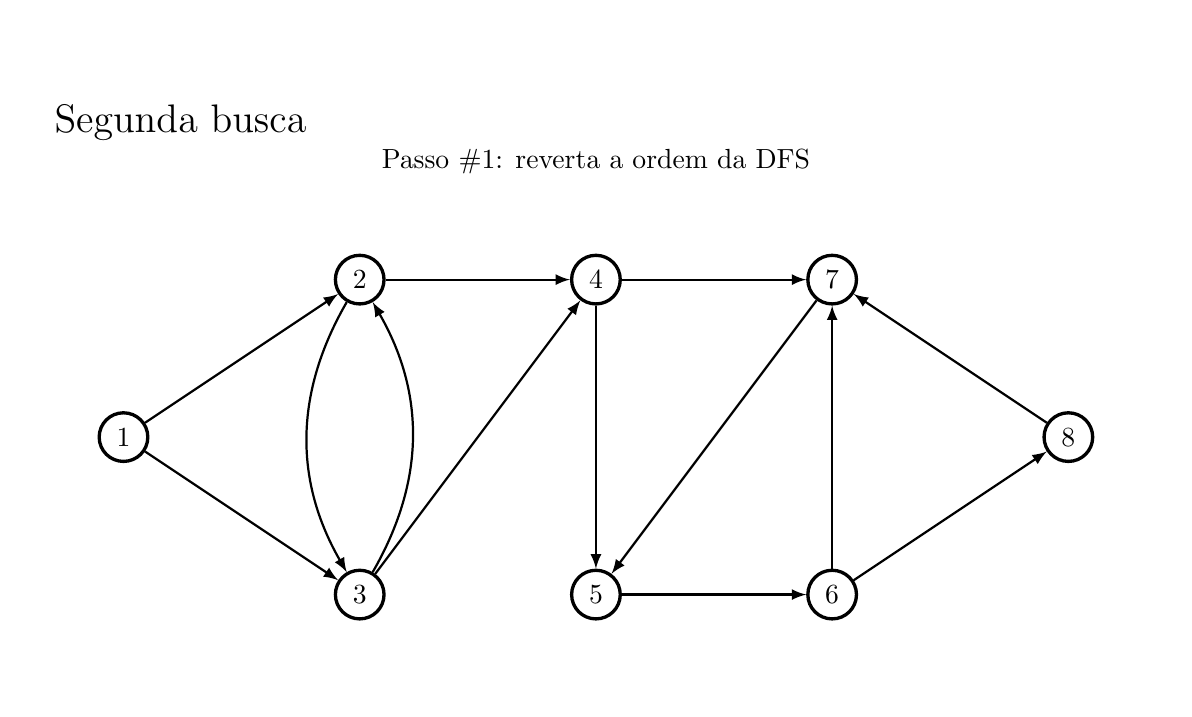
\begin{tikzpicture}
\node[draw,opacity=0] at (0, 0) {x};
\node[draw,opacity=0] at (14, 8) {x};

	\node[anchor=west] (title) at (0.0, 7.0) { \Large \bbbold{Segunda busca} };

	\node[] (text) at (7.0, 6.5) { \bbtext{\bbbold{Passo \#1:} reverta a ordem da DFS} };


	\node[very thick,draw,circle] (node1) at (1.0, 3.0) { \bbtext{1} };

	\node[very thick,draw,circle] (node2) at (4.0, 5.0) { \bbtext{2} };

	\node[very thick,draw,circle] (node3) at (4.0, 1.0) { \bbtext{3} };

	\node[very thick,draw,circle] (node4) at (7.0, 5.0) { \bbtext{4} };

	\node[very thick,draw,circle] (node5) at (7.0, 1.0) { \bbtext{5} };

	\node[very thick,draw,circle] (node7) at (10.0, 5.0) { \bbtext{7} };

	\node[very thick,draw,circle] (node6) at (10.0, 1.0) { \bbtext{6} };

	\node[very thick,draw,circle] (node8) at (13.0, 3.0) { \bbtext{8} };

	\draw[thick,-latex](node1) to (node2);

	\draw[thick,-latex](node1) to (node3);

	\draw[thick,-latex](node3) to [bend right] (node2);

	\draw[thick,-latex](node2) to [bend right] (node3);

	\draw[thick,-latex](node2) to (node4);

	\draw[thick,-latex](node3) to (node4);

	\draw[thick,-latex](node4) to (node5);

	\draw[thick,-latex](node4) to (node7);

	\draw[thick,-latex](node5) to (node6);

	\draw[thick,-latex](node6) to (node7);

	\draw[thick,-latex](node6) to (node8);

	\draw[thick,-latex](node7) to (node5);

	\draw[thick,-latex](node8) to (node7);

\end{tikzpicture}
\end{frame}
\begin{frame}[plain,t]
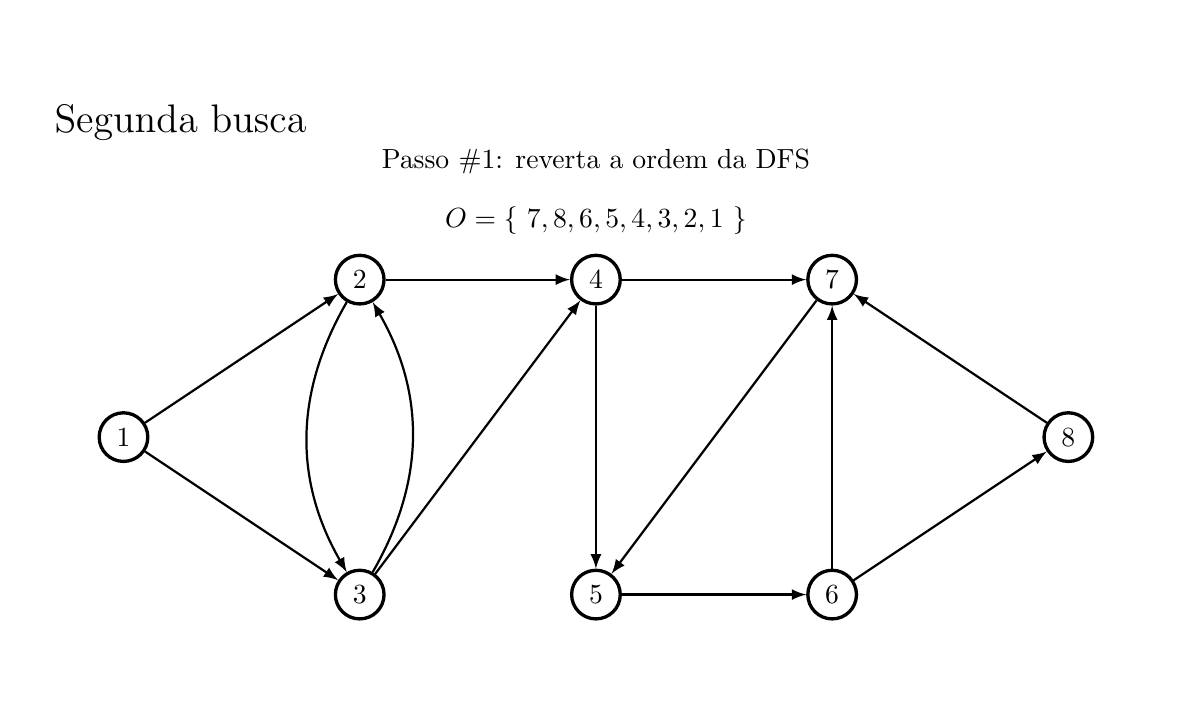
\begin{tikzpicture}
\node[draw,opacity=0] at (0, 0) {x};
\node[draw,opacity=0] at (14, 8) {x};

	\node[anchor=west] (title) at (0.0, 7.0) { \Large \bbbold{Segunda busca} };

	\node[] (text) at (7.0, 6.5) { \bbtext{\bbbold{Passo \#1:} reverta a ordem da DFS} };


	\node[very thick,draw,circle] (node1) at (1.0, 3.0) { \bbtext{1} };

	\node[very thick,draw,circle] (node2) at (4.0, 5.0) { \bbtext{2} };

	\node[very thick,draw,circle] (node3) at (4.0, 1.0) { \bbtext{3} };

	\node[very thick,draw,circle] (node4) at (7.0, 5.0) { \bbtext{4} };

	\node[very thick,draw,circle] (node5) at (7.0, 1.0) { \bbtext{5} };

	\node[very thick,draw,circle] (node7) at (10.0, 5.0) { \bbtext{7} };

	\node[very thick,draw,circle] (node6) at (10.0, 1.0) { \bbtext{6} };

	\node[very thick,draw,circle] (node8) at (13.0, 3.0) { \bbtext{8} };

	\draw[thick,-latex](node1) to (node2);

	\draw[thick,-latex](node1) to (node3);

	\draw[thick,-latex](node3) to [bend right] (node2);

	\draw[thick,-latex](node2) to [bend right] (node3);

	\draw[thick,-latex](node2) to (node4);

	\draw[thick,-latex](node3) to (node4);

	\draw[thick,-latex](node4) to (node5);

	\draw[thick,-latex](node4) to (node7);

	\draw[thick,-latex](node5) to (node6);

	\draw[thick,-latex](node6) to (node7);

	\draw[thick,-latex](node6) to (node8);

	\draw[thick,-latex](node7) to (node5);

	\draw[thick,-latex](node8) to (node7);


	\node[] (order) at (7.0, 5.75) { $O = \{\ 7, 8, 6, 5, 4, 3, 2, 1\ \}$ };

\end{tikzpicture}
\end{frame}
\begin{frame}[plain,t]
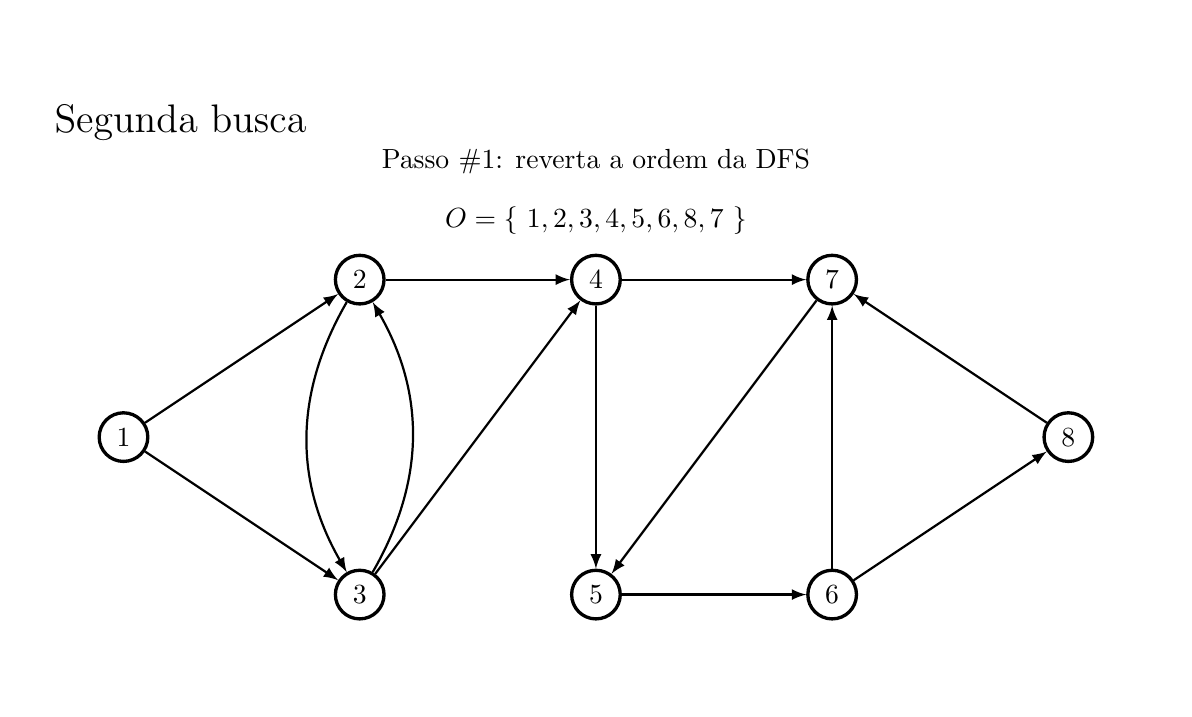
\begin{tikzpicture}
\node[draw,opacity=0] at (0, 0) {x};
\node[draw,opacity=0] at (14, 8) {x};

	\node[anchor=west] (title) at (0.0, 7.0) { \Large \bbbold{Segunda busca} };

	\node[] (text) at (7.0, 6.5) { \bbtext{\bbbold{Passo \#1:} reverta a ordem da DFS} };


	\node[very thick,draw,circle] (node1) at (1.0, 3.0) { \bbtext{1} };

	\node[very thick,draw,circle] (node2) at (4.0, 5.0) { \bbtext{2} };

	\node[very thick,draw,circle] (node3) at (4.0, 1.0) { \bbtext{3} };

	\node[very thick,draw,circle] (node4) at (7.0, 5.0) { \bbtext{4} };

	\node[very thick,draw,circle] (node5) at (7.0, 1.0) { \bbtext{5} };

	\node[very thick,draw,circle] (node7) at (10.0, 5.0) { \bbtext{7} };

	\node[very thick,draw,circle] (node6) at (10.0, 1.0) { \bbtext{6} };

	\node[very thick,draw,circle] (node8) at (13.0, 3.0) { \bbtext{8} };

	\draw[thick,-latex](node1) to (node2);

	\draw[thick,-latex](node1) to (node3);

	\draw[thick,-latex](node3) to [bend right] (node2);

	\draw[thick,-latex](node2) to [bend right] (node3);

	\draw[thick,-latex](node2) to (node4);

	\draw[thick,-latex](node3) to (node4);

	\draw[thick,-latex](node4) to (node5);

	\draw[thick,-latex](node4) to (node7);

	\draw[thick,-latex](node5) to (node6);

	\draw[thick,-latex](node6) to (node7);

	\draw[thick,-latex](node6) to (node8);

	\draw[thick,-latex](node7) to (node5);

	\draw[thick,-latex](node8) to (node7);


	\node[] (order) at (7.0, 5.75) { $O = \{\ 1, 2, 3, 4, 5, 6, 8, 7\ \}$ };


\end{tikzpicture}
\end{frame}
\begin{frame}[plain,t]
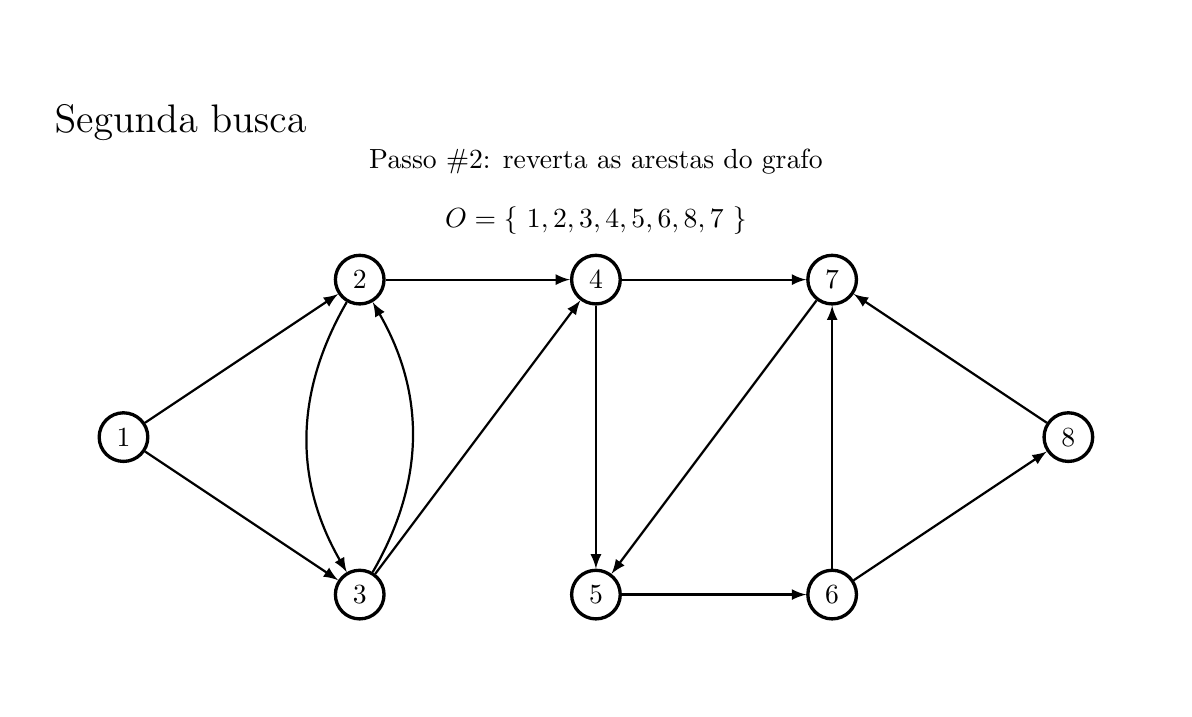
\begin{tikzpicture}
\node[draw,opacity=0] at (0, 0) {x};
\node[draw,opacity=0] at (14, 8) {x};

	\node[anchor=west] (title) at (0.0, 7.0) { \Large \bbbold{Segunda busca} };

	\node[] (text) at (7.0, 6.5) { \bbtext{\bbbold{Passo \#2:} reverta as arestas do grafo} };


	\node[very thick,draw,circle] (node1) at (1.0, 3.0) { \bbtext{1} };

	\node[very thick,draw,circle] (node2) at (4.0, 5.0) { \bbtext{2} };

	\node[very thick,draw,circle] (node3) at (4.0, 1.0) { \bbtext{3} };

	\node[very thick,draw,circle] (node4) at (7.0, 5.0) { \bbtext{4} };

	\node[very thick,draw,circle] (node5) at (7.0, 1.0) { \bbtext{5} };

	\node[very thick,draw,circle] (node7) at (10.0, 5.0) { \bbtext{7} };

	\node[very thick,draw,circle] (node6) at (10.0, 1.0) { \bbtext{6} };

	\node[very thick,draw,circle] (node8) at (13.0, 3.0) { \bbtext{8} };

	\draw[thick,-latex](node1) to (node2);

	\draw[thick,-latex](node1) to (node3);

	\draw[thick,-latex](node3) to [bend right] (node2);

	\draw[thick,-latex](node2) to [bend right] (node3);

	\draw[thick,-latex](node2) to (node4);

	\draw[thick,-latex](node3) to (node4);

	\draw[thick,-latex](node4) to (node5);

	\draw[thick,-latex](node4) to (node7);

	\draw[thick,-latex](node5) to (node6);

	\draw[thick,-latex](node6) to (node7);

	\draw[thick,-latex](node6) to (node8);

	\draw[thick,-latex](node7) to (node5);

	\draw[thick,-latex](node8) to (node7);


	\node[] (order) at (7.0, 5.75) { $O = \{\ 1, 2, 3, 4, 5, 6, 8, 7\ \}$ };



\end{tikzpicture}
\end{frame}
\begin{frame}[plain,t]
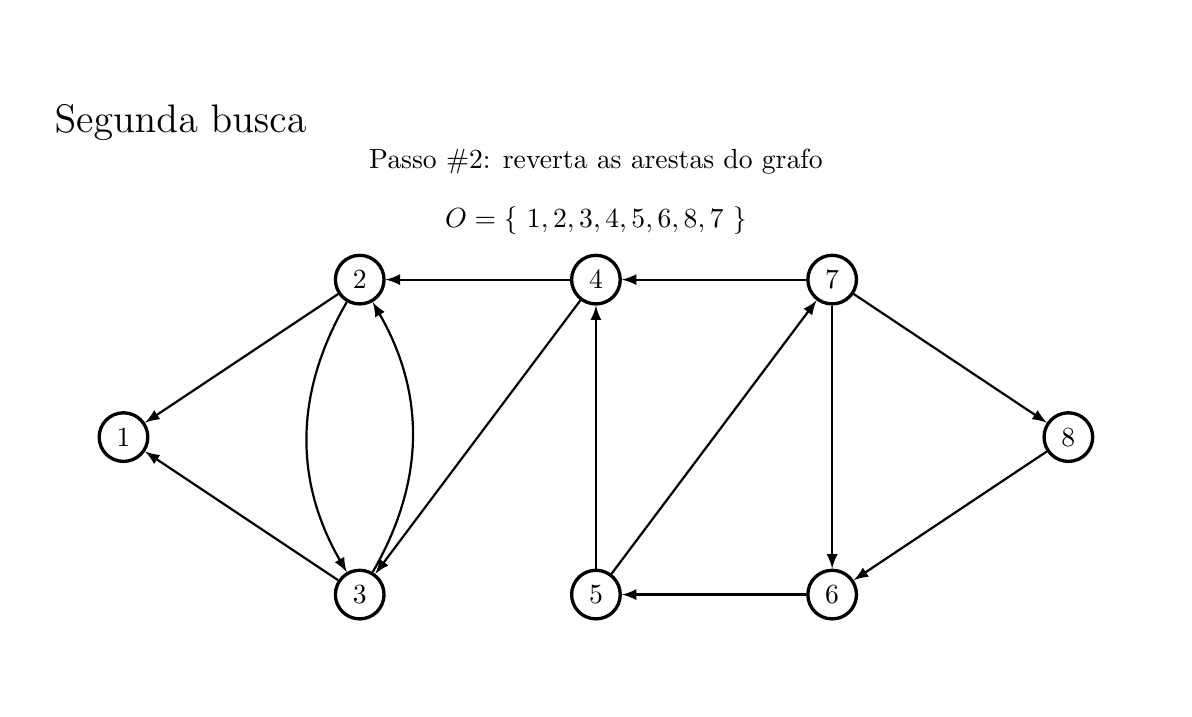
\begin{tikzpicture}
\node[draw,opacity=0] at (0, 0) {x};
\node[draw,opacity=0] at (14, 8) {x};

	\node[anchor=west] (title) at (0.0, 7.0) { \Large \bbbold{Segunda busca} };

	\node[] (text) at (7.0, 6.5) { \bbtext{\bbbold{Passo \#2:} reverta as arestas do grafo} };


	\node[very thick,draw,circle] (node1) at (1.0, 3.0) { \bbtext{1} };

	\node[very thick,draw,circle] (node2) at (4.0, 5.0) { \bbtext{2} };

	\node[very thick,draw,circle] (node3) at (4.0, 1.0) { \bbtext{3} };

	\node[very thick,draw,circle] (node4) at (7.0, 5.0) { \bbtext{4} };

	\node[very thick,draw,circle] (node5) at (7.0, 1.0) { \bbtext{5} };

	\node[very thick,draw,circle] (node7) at (10.0, 5.0) { \bbtext{7} };

	\node[very thick,draw,circle] (node6) at (10.0, 1.0) { \bbtext{6} };

	\node[very thick,draw,circle] (node8) at (13.0, 3.0) { \bbtext{8} };

	\draw[thick,-latex](node2) to (node1);

	\draw[thick,-latex](node3) to (node1);

	\draw[thick,-latex](node3) to [bend right] (node2);

	\draw[thick,-latex](node2) to [bend right] (node3);

	\draw[thick,-latex](node4) to (node2);

	\draw[thick,-latex](node4) to (node3);

	\draw[thick,-latex](node5) to (node4);

	\draw[thick,-latex](node7) to (node4);

	\draw[thick,-latex](node6) to (node5);

	\draw[thick,-latex](node7) to (node6);

	\draw[thick,-latex](node8) to (node6);

	\draw[thick,-latex](node5) to (node7);

	\draw[thick,-latex](node7) to (node8);


	\node[] (order) at (7.0, 5.75) { $O = \{\ 1, 2, 3, 4, 5, 6, 8, 7\ \}$ };


















\end{tikzpicture}
\end{frame}
\begin{frame}[plain,t]
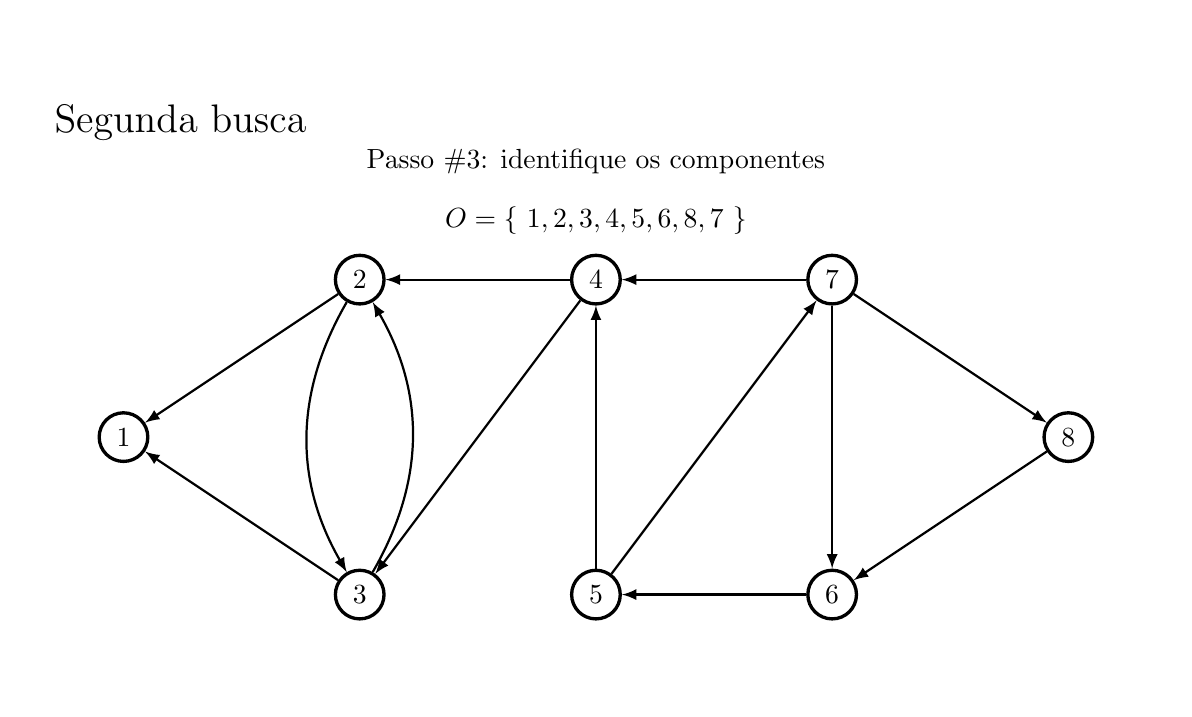
\begin{tikzpicture}
\node[draw,opacity=0] at (0, 0) {x};
\node[draw,opacity=0] at (14, 8) {x};

	\node[anchor=west] (title) at (0.0, 7.0) { \Large \bbbold{Segunda busca} };

	\node[] (text) at (7.0, 6.5) { \bbtext{\bbbold{Passo \#3:} identifique os componentes} };


	\node[very thick,draw,circle] (node1) at (1.0, 3.0) { \bbtext{1} };

	\node[very thick,draw,circle] (node2) at (4.0, 5.0) { \bbtext{2} };

	\node[very thick,draw,circle] (node3) at (4.0, 1.0) { \bbtext{3} };

	\node[very thick,draw,circle] (node4) at (7.0, 5.0) { \bbtext{4} };

	\node[very thick,draw,circle] (node5) at (7.0, 1.0) { \bbtext{5} };

	\node[very thick,draw,circle] (node7) at (10.0, 5.0) { \bbtext{7} };

	\node[very thick,draw,circle] (node6) at (10.0, 1.0) { \bbtext{6} };

	\node[very thick,draw,circle] (node8) at (13.0, 3.0) { \bbtext{8} };

	\draw[thick,-latex](node2) to (node1);

	\draw[thick,-latex](node3) to (node1);

	\draw[thick,-latex](node3) to [bend right] (node2);

	\draw[thick,-latex](node2) to [bend right] (node3);

	\draw[thick,-latex](node4) to (node2);

	\draw[thick,-latex](node4) to (node3);

	\draw[thick,-latex](node5) to (node4);

	\draw[thick,-latex](node7) to (node4);

	\draw[thick,-latex](node6) to (node5);

	\draw[thick,-latex](node7) to (node6);

	\draw[thick,-latex](node8) to (node6);

	\draw[thick,-latex](node5) to (node7);

	\draw[thick,-latex](node7) to (node8);


	\node[] (order) at (7.0, 5.75) { $O = \{\ 1, 2, 3, 4, 5, 6, 8, 7\ \}$ };



















\end{tikzpicture}
\end{frame}
\begin{frame}[plain,t]
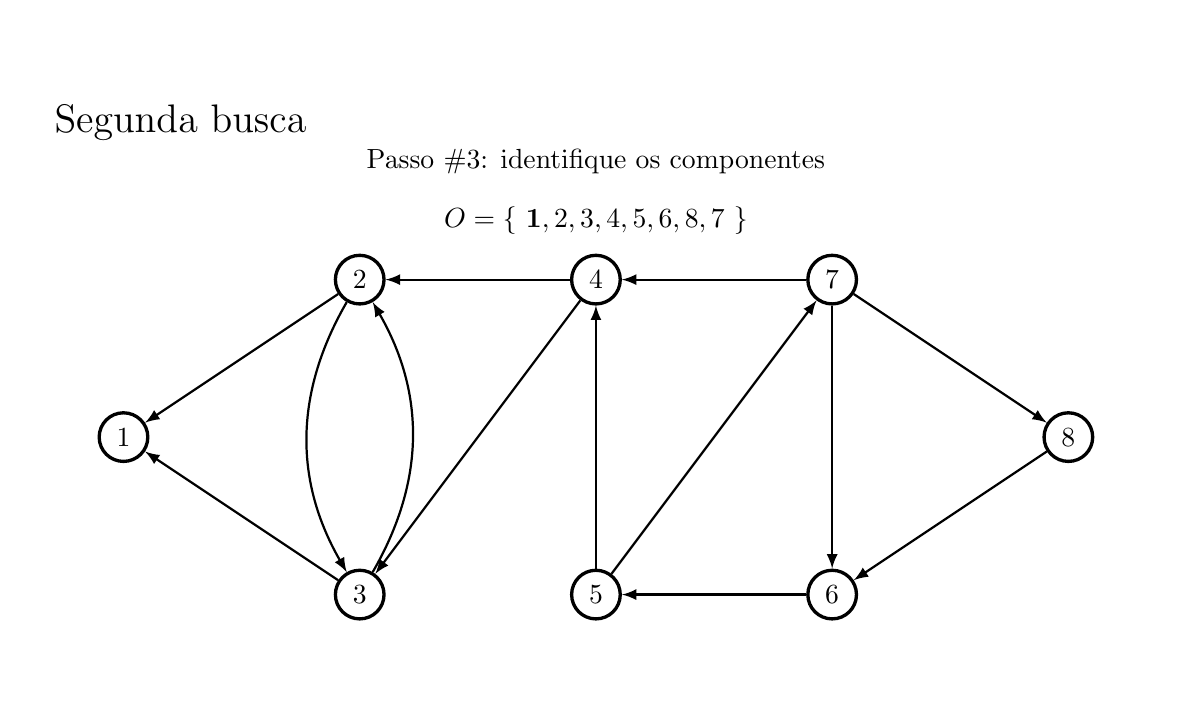
\begin{tikzpicture}
\node[draw,opacity=0] at (0, 0) {x};
\node[draw,opacity=0] at (14, 8) {x};

	\node[anchor=west] (title) at (0.0, 7.0) { \Large \bbbold{Segunda busca} };

	\node[] (text) at (7.0, 6.5) { \bbtext{\bbbold{Passo \#3:} identifique os componentes} };


	\node[very thick,draw,circle] (node1) at (1.0, 3.0) { \bbtext{1} };

	\node[very thick,draw,circle] (node2) at (4.0, 5.0) { \bbtext{2} };

	\node[very thick,draw,circle] (node3) at (4.0, 1.0) { \bbtext{3} };

	\node[very thick,draw,circle] (node4) at (7.0, 5.0) { \bbtext{4} };

	\node[very thick,draw,circle] (node5) at (7.0, 1.0) { \bbtext{5} };

	\node[very thick,draw,circle] (node7) at (10.0, 5.0) { \bbtext{7} };

	\node[very thick,draw,circle] (node6) at (10.0, 1.0) { \bbtext{6} };

	\node[very thick,draw,circle] (node8) at (13.0, 3.0) { \bbtext{8} };

	\draw[thick,-latex](node2) to (node1);

	\draw[thick,-latex](node3) to (node1);

	\draw[thick,-latex](node3) to [bend right] (node2);

	\draw[thick,-latex](node2) to [bend right] (node3);

	\draw[thick,-latex](node4) to (node2);

	\draw[thick,-latex](node4) to (node3);

	\draw[thick,-latex](node5) to (node4);

	\draw[thick,-latex](node7) to (node4);

	\draw[thick,-latex](node6) to (node5);

	\draw[thick,-latex](node7) to (node6);

	\draw[thick,-latex](node8) to (node6);

	\draw[thick,-latex](node5) to (node7);

	\draw[thick,-latex](node7) to (node8);


	\node[] (order) at (7.0, 5.75) { $O = \{\ \mathbf{1}, 2, 3, 4, 5, 6, 8, 7\ \}$ };




















\end{tikzpicture}
\end{frame}
\begin{frame}[plain,t]
\begin{tikzpicture}
\node[draw,opacity=0] at (0, 0) {x};
\node[draw,opacity=0] at (14, 8) {x};

	\node[anchor=west] (title) at (0.0, 7.0) { \Large \bbbold{Segunda busca} };

	\node[] (text) at (7.0, 6.5) { \bbtext{\bbbold{Passo \#3:} identifique os componentes} };


	\node[very thick,draw,circle,fill=BBCyan] (node1) at (1.0, 3.0) { \bbtext{1} };

	\node[very thick,draw,circle] (node2) at (4.0, 5.0) { \bbtext{2} };

	\node[very thick,draw,circle] (node3) at (4.0, 1.0) { \bbtext{3} };

	\node[very thick,draw,circle] (node4) at (7.0, 5.0) { \bbtext{4} };

	\node[very thick,draw,circle] (node5) at (7.0, 1.0) { \bbtext{5} };

	\node[very thick,draw,circle] (node7) at (10.0, 5.0) { \bbtext{7} };

	\node[very thick,draw,circle] (node6) at (10.0, 1.0) { \bbtext{6} };

	\node[very thick,draw,circle] (node8) at (13.0, 3.0) { \bbtext{8} };

	\draw[thick,-latex](node2) to (node1);

	\draw[thick,-latex](node3) to (node1);

	\draw[thick,-latex](node3) to [bend right] (node2);

	\draw[thick,-latex](node2) to [bend right] (node3);

	\draw[thick,-latex](node4) to (node2);

	\draw[thick,-latex](node4) to (node3);

	\draw[thick,-latex](node5) to (node4);

	\draw[thick,-latex](node7) to (node4);

	\draw[thick,-latex](node6) to (node5);

	\draw[thick,-latex](node7) to (node6);

	\draw[thick,-latex](node8) to (node6);

	\draw[thick,-latex](node5) to (node7);

	\draw[thick,-latex](node7) to (node8);


	\node[] (order) at (7.0, 5.75) { $O = \{\ \mathbf{1}, 2, 3, 4, 5, 6, 8, 7\ \}$ };





















\end{tikzpicture}
\end{frame}
\begin{frame}[plain,t]
\begin{tikzpicture}
\node[draw,opacity=0] at (0, 0) {x};
\node[draw,opacity=0] at (14, 8) {x};

	\node[anchor=west] (title) at (0.0, 7.0) { \Large \bbbold{Segunda busca} };

	\node[] (text) at (7.0, 6.5) { \bbtext{\bbbold{Passo \#3:} identifique os componentes} };


	\node[very thick,draw,circle,fill=BBCyan] (node1) at (1.0, 3.0) { \bbtext{1} };

	\node[very thick,draw,circle] (node2) at (4.0, 5.0) { \bbtext{2} };

	\node[very thick,draw,circle] (node3) at (4.0, 1.0) { \bbtext{3} };

	\node[very thick,draw,circle] (node4) at (7.0, 5.0) { \bbtext{4} };

	\node[very thick,draw,circle] (node5) at (7.0, 1.0) { \bbtext{5} };

	\node[very thick,draw,circle] (node7) at (10.0, 5.0) { \bbtext{7} };

	\node[very thick,draw,circle] (node6) at (10.0, 1.0) { \bbtext{6} };

	\node[very thick,draw,circle] (node8) at (13.0, 3.0) { \bbtext{8} };

	\draw[thick,-latex](node2) to (node1);

	\draw[thick,-latex](node3) to (node1);

	\draw[thick,-latex](node3) to [bend right] (node2);

	\draw[thick,-latex](node2) to [bend right] (node3);

	\draw[thick,-latex](node4) to (node2);

	\draw[thick,-latex](node4) to (node3);

	\draw[thick,-latex](node5) to (node4);

	\draw[thick,-latex](node7) to (node4);

	\draw[thick,-latex](node6) to (node5);

	\draw[thick,-latex](node7) to (node6);

	\draw[thick,-latex](node8) to (node6);

	\draw[thick,-latex](node5) to (node7);

	\draw[thick,-latex](node7) to (node8);


	\node[] (order) at (7.0, 5.75) { $O = \{\ 1, \mathbf{2}, 3, 4, 5, 6, 8, 7\ \}$ };






















\end{tikzpicture}
\end{frame}
\begin{frame}[plain,t]
\begin{tikzpicture}
\node[draw,opacity=0] at (0, 0) {x};
\node[draw,opacity=0] at (14, 8) {x};

	\node[anchor=west] (title) at (0.0, 7.0) { \Large \bbbold{Segunda busca} };

	\node[] (text) at (7.0, 6.5) { \bbtext{\bbbold{Passo \#3:} identifique os componentes} };


	\node[very thick,draw,circle,fill=BBCyan] (node1) at (1.0, 3.0) { \bbtext{1} };

	\node[very thick,draw,circle,fill=BBGreen] (node2) at (4.0, 5.0) { \bbtext{2} };

	\node[very thick,draw,circle] (node3) at (4.0, 1.0) { \bbtext{3} };

	\node[very thick,draw,circle] (node4) at (7.0, 5.0) { \bbtext{4} };

	\node[very thick,draw,circle] (node5) at (7.0, 1.0) { \bbtext{5} };

	\node[very thick,draw,circle] (node7) at (10.0, 5.0) { \bbtext{7} };

	\node[very thick,draw,circle] (node6) at (10.0, 1.0) { \bbtext{6} };

	\node[very thick,draw,circle] (node8) at (13.0, 3.0) { \bbtext{8} };

	\draw[thick,-latex](node2) to (node1);

	\draw[thick,-latex](node3) to (node1);

	\draw[thick,-latex](node3) to [bend right] (node2);

	\draw[thick,-latex](node2) to [bend right] (node3);

	\draw[thick,-latex](node4) to (node2);

	\draw[thick,-latex](node4) to (node3);

	\draw[thick,-latex](node5) to (node4);

	\draw[thick,-latex](node7) to (node4);

	\draw[thick,-latex](node6) to (node5);

	\draw[thick,-latex](node7) to (node6);

	\draw[thick,-latex](node8) to (node6);

	\draw[thick,-latex](node5) to (node7);

	\draw[thick,-latex](node7) to (node8);


	\node[] (order) at (7.0, 5.75) { $O = \{\ 1, \mathbf{2}, 3, 4, 5, 6, 8, 7\ \}$ };























\end{tikzpicture}
\end{frame}
\begin{frame}[plain,t]
\begin{tikzpicture}
\node[draw,opacity=0] at (0, 0) {x};
\node[draw,opacity=0] at (14, 8) {x};

	\node[anchor=west] (title) at (0.0, 7.0) { \Large \bbbold{Segunda busca} };

	\node[] (text) at (7.0, 6.5) { \bbtext{\bbbold{Passo \#3:} identifique os componentes} };


	\node[very thick,draw,circle,fill=BBCyan] (node1) at (1.0, 3.0) { \bbtext{1} };

	\node[very thick,draw,circle,fill=BBGreen] (node2) at (4.0, 5.0) { \bbtext{2} };

	\node[very thick,draw,circle,fill=BBGreen] (node3) at (4.0, 1.0) { \bbtext{3} };

	\node[very thick,draw,circle] (node4) at (7.0, 5.0) { \bbtext{4} };

	\node[very thick,draw,circle] (node5) at (7.0, 1.0) { \bbtext{5} };

	\node[very thick,draw,circle] (node7) at (10.0, 5.0) { \bbtext{7} };

	\node[very thick,draw,circle] (node6) at (10.0, 1.0) { \bbtext{6} };

	\node[very thick,draw,circle] (node8) at (13.0, 3.0) { \bbtext{8} };

	\draw[thick,-latex](node2) to (node1);

	\draw[thick,-latex](node3) to (node1);

	\draw[thick,-latex](node3) to [bend right] (node2);

	\draw[thick,-latex](node2) to [bend right] (node3);

	\draw[thick,-latex](node4) to (node2);

	\draw[thick,-latex](node4) to (node3);

	\draw[thick,-latex](node5) to (node4);

	\draw[thick,-latex](node7) to (node4);

	\draw[thick,-latex](node6) to (node5);

	\draw[thick,-latex](node7) to (node6);

	\draw[thick,-latex](node8) to (node6);

	\draw[thick,-latex](node5) to (node7);

	\draw[thick,-latex](node7) to (node8);


	\node[] (order) at (7.0, 5.75) { $O = \{\ 1, \mathbf{2}, 3, 4, 5, 6, 8, 7\ \}$ };
























\end{tikzpicture}
\end{frame}
\begin{frame}[plain,t]
\begin{tikzpicture}
\node[draw,opacity=0] at (0, 0) {x};
\node[draw,opacity=0] at (14, 8) {x};

	\node[anchor=west] (title) at (0.0, 7.0) { \Large \bbbold{Segunda busca} };

	\node[] (text) at (7.0, 6.5) { \bbtext{\bbbold{Passo \#3:} identifique os componentes} };


	\node[very thick,draw,circle,fill=BBCyan] (node1) at (1.0, 3.0) { \bbtext{1} };

	\node[very thick,draw,circle,fill=BBGreen] (node2) at (4.0, 5.0) { \bbtext{2} };

	\node[very thick,draw,circle,fill=BBGreen] (node3) at (4.0, 1.0) { \bbtext{3} };

	\node[very thick,draw,circle] (node4) at (7.0, 5.0) { \bbtext{4} };

	\node[very thick,draw,circle] (node5) at (7.0, 1.0) { \bbtext{5} };

	\node[very thick,draw,circle] (node7) at (10.0, 5.0) { \bbtext{7} };

	\node[very thick,draw,circle] (node6) at (10.0, 1.0) { \bbtext{6} };

	\node[very thick,draw,circle] (node8) at (13.0, 3.0) { \bbtext{8} };

	\draw[thick,-latex](node2) to (node1);

	\draw[thick,-latex](node3) to (node1);

	\draw[thick,-latex](node3) to [bend right] (node2);

	\draw[thick,-latex](node2) to [bend right] (node3);

	\draw[thick,-latex](node4) to (node2);

	\draw[thick,-latex](node4) to (node3);

	\draw[thick,-latex](node5) to (node4);

	\draw[thick,-latex](node7) to (node4);

	\draw[thick,-latex](node6) to (node5);

	\draw[thick,-latex](node7) to (node6);

	\draw[thick,-latex](node8) to (node6);

	\draw[thick,-latex](node5) to (node7);

	\draw[thick,-latex](node7) to (node8);


	\node[] (order) at (7.0, 5.75) { $O = \{\ 1, 2, 3, \mathbf{4}, 5, 6, 8, 7\ \}$ };

























\end{tikzpicture}
\end{frame}
\begin{frame}[plain,t]
\begin{tikzpicture}
\node[draw,opacity=0] at (0, 0) {x};
\node[draw,opacity=0] at (14, 8) {x};

	\node[anchor=west] (title) at (0.0, 7.0) { \Large \bbbold{Segunda busca} };

	\node[] (text) at (7.0, 6.5) { \bbtext{\bbbold{Passo \#3:} identifique os componentes} };


	\node[very thick,draw,circle,fill=BBCyan] (node1) at (1.0, 3.0) { \bbtext{1} };

	\node[very thick,draw,circle,fill=BBGreen] (node2) at (4.0, 5.0) { \bbtext{2} };

	\node[very thick,draw,circle,fill=BBGreen] (node3) at (4.0, 1.0) { \bbtext{3} };

	\node[very thick,draw,circle,fill=BBViolet] (node4) at (7.0, 5.0) { \bbtext{4} };

	\node[very thick,draw,circle] (node5) at (7.0, 1.0) { \bbtext{5} };

	\node[very thick,draw,circle] (node7) at (10.0, 5.0) { \bbtext{7} };

	\node[very thick,draw,circle] (node6) at (10.0, 1.0) { \bbtext{6} };

	\node[very thick,draw,circle] (node8) at (13.0, 3.0) { \bbtext{8} };

	\draw[thick,-latex](node2) to (node1);

	\draw[thick,-latex](node3) to (node1);

	\draw[thick,-latex](node3) to [bend right] (node2);

	\draw[thick,-latex](node2) to [bend right] (node3);

	\draw[thick,-latex](node4) to (node2);

	\draw[thick,-latex](node4) to (node3);

	\draw[thick,-latex](node5) to (node4);

	\draw[thick,-latex](node7) to (node4);

	\draw[thick,-latex](node6) to (node5);

	\draw[thick,-latex](node7) to (node6);

	\draw[thick,-latex](node8) to (node6);

	\draw[thick,-latex](node5) to (node7);

	\draw[thick,-latex](node7) to (node8);


	\node[] (order) at (7.0, 5.75) { $O = \{\ 1, 2, 3, \mathbf{4}, 5, 6, 8, 7\ \}$ };


























\end{tikzpicture}
\end{frame}
\begin{frame}[plain,t]
\begin{tikzpicture}
\node[draw,opacity=0] at (0, 0) {x};
\node[draw,opacity=0] at (14, 8) {x};

	\node[anchor=west] (title) at (0.0, 7.0) { \Large \bbbold{Segunda busca} };

	\node[] (text) at (7.0, 6.5) { \bbtext{\bbbold{Passo \#3:} identifique os componentes} };


	\node[very thick,draw,circle,fill=BBCyan] (node1) at (1.0, 3.0) { \bbtext{1} };

	\node[very thick,draw,circle,fill=BBGreen] (node2) at (4.0, 5.0) { \bbtext{2} };

	\node[very thick,draw,circle,fill=BBGreen] (node3) at (4.0, 1.0) { \bbtext{3} };

	\node[very thick,draw,circle,fill=BBViolet] (node4) at (7.0, 5.0) { \bbtext{4} };

	\node[very thick,draw,circle] (node5) at (7.0, 1.0) { \bbtext{5} };

	\node[very thick,draw,circle] (node7) at (10.0, 5.0) { \bbtext{7} };

	\node[very thick,draw,circle] (node6) at (10.0, 1.0) { \bbtext{6} };

	\node[very thick,draw,circle] (node8) at (13.0, 3.0) { \bbtext{8} };

	\draw[thick,-latex](node2) to (node1);

	\draw[thick,-latex](node3) to (node1);

	\draw[thick,-latex](node3) to [bend right] (node2);

	\draw[thick,-latex](node2) to [bend right] (node3);

	\draw[thick,-latex](node4) to (node2);

	\draw[thick,-latex](node4) to (node3);

	\draw[thick,-latex](node5) to (node4);

	\draw[thick,-latex](node7) to (node4);

	\draw[thick,-latex](node6) to (node5);

	\draw[thick,-latex](node7) to (node6);

	\draw[thick,-latex](node8) to (node6);

	\draw[thick,-latex](node5) to (node7);

	\draw[thick,-latex](node7) to (node8);


	\node[] (order) at (7.0, 5.75) { $O = \{\ 1, 2, 3, 4, \mathbf{5}, 6, 8, 7\ \}$ };



























\end{tikzpicture}
\end{frame}
\begin{frame}[plain,t]
\begin{tikzpicture}
\node[draw,opacity=0] at (0, 0) {x};
\node[draw,opacity=0] at (14, 8) {x};

	\node[anchor=west] (title) at (0.0, 7.0) { \Large \bbbold{Segunda busca} };

	\node[] (text) at (7.0, 6.5) { \bbtext{\bbbold{Passo \#3:} identifique os componentes} };


	\node[very thick,draw,circle,fill=BBCyan] (node1) at (1.0, 3.0) { \bbtext{1} };

	\node[very thick,draw,circle,fill=BBGreen] (node2) at (4.0, 5.0) { \bbtext{2} };

	\node[very thick,draw,circle,fill=BBGreen] (node3) at (4.0, 1.0) { \bbtext{3} };

	\node[very thick,draw,circle,fill=BBViolet] (node4) at (7.0, 5.0) { \bbtext{4} };

	\node[very thick,draw,circle,fill=BBOrange] (node5) at (7.0, 1.0) { \bbtext{5} };

	\node[very thick,draw,circle] (node7) at (10.0, 5.0) { \bbtext{7} };

	\node[very thick,draw,circle] (node6) at (10.0, 1.0) { \bbtext{6} };

	\node[very thick,draw,circle] (node8) at (13.0, 3.0) { \bbtext{8} };

	\draw[thick,-latex](node2) to (node1);

	\draw[thick,-latex](node3) to (node1);

	\draw[thick,-latex](node3) to [bend right] (node2);

	\draw[thick,-latex](node2) to [bend right] (node3);

	\draw[thick,-latex](node4) to (node2);

	\draw[thick,-latex](node4) to (node3);

	\draw[thick,-latex](node5) to (node4);

	\draw[thick,-latex](node7) to (node4);

	\draw[thick,-latex](node6) to (node5);

	\draw[thick,-latex](node7) to (node6);

	\draw[thick,-latex](node8) to (node6);

	\draw[thick,-latex](node5) to (node7);

	\draw[thick,-latex](node7) to (node8);


	\node[] (order) at (7.0, 5.75) { $O = \{\ 1, 2, 3, 4, \mathbf{5}, 6, 8, 7\ \}$ };




























\end{tikzpicture}
\end{frame}
\begin{frame}[plain,t]
\begin{tikzpicture}
\node[draw,opacity=0] at (0, 0) {x};
\node[draw,opacity=0] at (14, 8) {x};

	\node[anchor=west] (title) at (0.0, 7.0) { \Large \bbbold{Segunda busca} };

	\node[] (text) at (7.0, 6.5) { \bbtext{\bbbold{Passo \#3:} identifique os componentes} };


	\node[very thick,draw,circle,fill=BBCyan] (node1) at (1.0, 3.0) { \bbtext{1} };

	\node[very thick,draw,circle,fill=BBGreen] (node2) at (4.0, 5.0) { \bbtext{2} };

	\node[very thick,draw,circle,fill=BBGreen] (node3) at (4.0, 1.0) { \bbtext{3} };

	\node[very thick,draw,circle,fill=BBViolet] (node4) at (7.0, 5.0) { \bbtext{4} };

	\node[very thick,draw,circle,fill=BBOrange] (node5) at (7.0, 1.0) { \bbtext{5} };

	\node[very thick,draw,circle,fill=BBOrange] (node7) at (10.0, 5.0) { \bbtext{7} };

	\node[very thick,draw,circle] (node6) at (10.0, 1.0) { \bbtext{6} };

	\node[very thick,draw,circle] (node8) at (13.0, 3.0) { \bbtext{8} };

	\draw[thick,-latex](node2) to (node1);

	\draw[thick,-latex](node3) to (node1);

	\draw[thick,-latex](node3) to [bend right] (node2);

	\draw[thick,-latex](node2) to [bend right] (node3);

	\draw[thick,-latex](node4) to (node2);

	\draw[thick,-latex](node4) to (node3);

	\draw[thick,-latex](node5) to (node4);

	\draw[thick,-latex](node7) to (node4);

	\draw[thick,-latex](node6) to (node5);

	\draw[thick,-latex](node7) to (node6);

	\draw[thick,-latex](node8) to (node6);

	\draw[thick,-latex](node5) to (node7);

	\draw[thick,-latex](node7) to (node8);


	\node[] (order) at (7.0, 5.75) { $O = \{\ 1, 2, 3, 4, \mathbf{5}, 6, 8, 7\ \}$ };





























\end{tikzpicture}
\end{frame}
\begin{frame}[plain,t]
\begin{tikzpicture}
\node[draw,opacity=0] at (0, 0) {x};
\node[draw,opacity=0] at (14, 8) {x};

	\node[anchor=west] (title) at (0.0, 7.0) { \Large \bbbold{Segunda busca} };

	\node[] (text) at (7.0, 6.5) { \bbtext{\bbbold{Passo \#3:} identifique os componentes} };


	\node[very thick,draw,circle,fill=BBCyan] (node1) at (1.0, 3.0) { \bbtext{1} };

	\node[very thick,draw,circle,fill=BBGreen] (node2) at (4.0, 5.0) { \bbtext{2} };

	\node[very thick,draw,circle,fill=BBGreen] (node3) at (4.0, 1.0) { \bbtext{3} };

	\node[very thick,draw,circle,fill=BBViolet] (node4) at (7.0, 5.0) { \bbtext{4} };

	\node[very thick,draw,circle,fill=BBOrange] (node5) at (7.0, 1.0) { \bbtext{5} };

	\node[very thick,draw,circle,fill=BBOrange] (node7) at (10.0, 5.0) { \bbtext{7} };

	\node[very thick,draw,circle] (node6) at (10.0, 1.0) { \bbtext{6} };

	\node[very thick,draw,circle,fill=BBOrange] (node8) at (13.0, 3.0) { \bbtext{8} };

	\draw[thick,-latex](node2) to (node1);

	\draw[thick,-latex](node3) to (node1);

	\draw[thick,-latex](node3) to [bend right] (node2);

	\draw[thick,-latex](node2) to [bend right] (node3);

	\draw[thick,-latex](node4) to (node2);

	\draw[thick,-latex](node4) to (node3);

	\draw[thick,-latex](node5) to (node4);

	\draw[thick,-latex](node7) to (node4);

	\draw[thick,-latex](node6) to (node5);

	\draw[thick,-latex](node7) to (node6);

	\draw[thick,-latex](node8) to (node6);

	\draw[thick,-latex](node5) to (node7);

	\draw[thick,-latex](node7) to (node8);


	\node[] (order) at (7.0, 5.75) { $O = \{\ 1, 2, 3, 4, \mathbf{5}, 6, 8, 7\ \}$ };






























\end{tikzpicture}
\end{frame}
\begin{frame}[plain,t]
\begin{tikzpicture}
\node[draw,opacity=0] at (0, 0) {x};
\node[draw,opacity=0] at (14, 8) {x};

	\node[anchor=west] (title) at (0.0, 7.0) { \Large \bbbold{Segunda busca} };

	\node[] (text) at (7.0, 6.5) { \bbtext{\bbbold{Passo \#3:} identifique os componentes} };


	\node[very thick,draw,circle,fill=BBCyan] (node1) at (1.0, 3.0) { \bbtext{1} };

	\node[very thick,draw,circle,fill=BBGreen] (node2) at (4.0, 5.0) { \bbtext{2} };

	\node[very thick,draw,circle,fill=BBGreen] (node3) at (4.0, 1.0) { \bbtext{3} };

	\node[very thick,draw,circle,fill=BBViolet] (node4) at (7.0, 5.0) { \bbtext{4} };

	\node[very thick,draw,circle,fill=BBOrange] (node5) at (7.0, 1.0) { \bbtext{5} };

	\node[very thick,draw,circle,fill=BBOrange] (node7) at (10.0, 5.0) { \bbtext{7} };

	\node[very thick,draw,circle,fill=BBOrange] (node6) at (10.0, 1.0) { \bbtext{6} };

	\node[very thick,draw,circle,fill=BBOrange] (node8) at (13.0, 3.0) { \bbtext{8} };

	\draw[thick,-latex](node2) to (node1);

	\draw[thick,-latex](node3) to (node1);

	\draw[thick,-latex](node3) to [bend right] (node2);

	\draw[thick,-latex](node2) to [bend right] (node3);

	\draw[thick,-latex](node4) to (node2);

	\draw[thick,-latex](node4) to (node3);

	\draw[thick,-latex](node5) to (node4);

	\draw[thick,-latex](node7) to (node4);

	\draw[thick,-latex](node6) to (node5);

	\draw[thick,-latex](node7) to (node6);

	\draw[thick,-latex](node8) to (node6);

	\draw[thick,-latex](node5) to (node7);

	\draw[thick,-latex](node7) to (node8);


	\node[] (order) at (7.0, 5.75) { $O = \{\ 1, 2, 3, 4, \mathbf{5}, 6, 8, 7\ \}$ };































\end{tikzpicture}
\end{frame}
\begin{frame}[plain,t]

\inputsnippet{cpp}{45}{65}{codes/kosaraju.cpp}

\end{frame}
\begin{frame}[plain,t]

\inputsnippet{cpp}{33}{43}{codes/kosaraju.cpp}


\end{frame}
\begin{frame}[plain,t]
\begin{tikzpicture}
\node[draw,opacity=0] at (0, 0) {x};
\node[draw,opacity=0] at (14, 8) {x};

	\node[anchor=west] (title) at (0.0, 6.0) { \Large \bbbold{Referências} };

	\node[anchor=west] (b) at (1.0, 5.0) { $1.$ \bbbold{HALIM}, \bbtext{Felix}; \bbbold{HALIM}, \bbtext{Steve}. \bbenglish{Competitive Programming 3,} \bbtext{2010.} };

	\node[anchor=west] (c) at (1.0, 4.0) { $2.$ \bbbold{LAAKSONEN}, \bbtext{Antti}. \bbenglish{Competitive Programmer's Handbook,} \bbtext{2018.} };

\end{tikzpicture}
\end{frame}
\end{document}
